\documentclass[ebook,9pt,oneside,openany]{memoir}
\usepackage[utf8x]{inputenc}
\usepackage[english]{babel}
\usepackage{float}
\usepackage[backref=page]{hyperref}
\hypersetup{colorlinks, linktocpage, % hyperref customization
            linkcolor={blue!70!black}, % \sections, figures
            citecolor={blue!70!black}, % \cite
            urlcolor={black!100!black}
           }
\usepackage{amsmath,amsfonts,amssymb,amsthm}
\usepackage{url}
\usepackage{bbm}
\usepackage{subcaption}
\usepackage{multicol}
\usepackage{listings}
\usepackage{mwe}


%\usepackage{breqn}

\newtheorem{theorem}{Theorem}

\theoremstyle{definition}
\newtheorem{example}{Example}

\setlrmarginsandblock{1.5cm}{1.5cm}{*}
\setulmarginsandblock{2.5cm}{*}{1}
\checkandfixthelayout

\nouppercaseheads
\makepagestyle{mystyle}
\makeevenhead{mystyle}{\thepage}{}{}
\makeoddhead{mystyle}{}{}{\itshape\leftmark}
\makeevenfoot{mystyle}{}{}{}
\makeoddfoot{mystyle}{}{}{}
\makepsmarks{mystyle}{
  \createmark{chapter}{left}{nonumber}{}{}}

%%%%%%%%%%%%%%%%%%%%%%%%%%%%%%%%%%%%%%
%------Fonts (in order of beauty)
%--Jens De Pelsmaeker; takes more space, tildes are ok
%\usepackage[sc]{mathpazo}\usepackage[T1]{fontenc}\linespread{1.05} % Palladio needs more leading (space between lines)
%--David Plazas recommended; takes less space, tildes are too high
\usepackage{libertine} % Normal
%--Carlos Cuartas; too clear and reader might get bored
%\usepackage[T1]{fontenc}\usepackage{lmodern}
%--Arial
%\usepackage{helvet}\renewcommand{\familydefault}{\sfdefault} % It's ok
%%%%%%%%%%%%%%%%%%%%%%%%%%%%%%%%%%%%%%
\setlength{\parindent}{0in}
\setlength\parskip{1\baselineskip}
\setcounter{tocdepth}{2}
\newtheorem{exmp}{Example}
\setcounter{secnumdepth}{5}
\renewcommand{\thesubsubsection}{\Roman{subsubsection}.}
\usepackage{mathtools}
\DeclarePairedDelimiter{\ceil}{\lceil}{\rceil}
\allowdisplaybreaks

\usepackage[pages=some, placement=bottom]{background}
\backgroundsetup{
scale=1,
color=black,
opacity=0.175,
angle=0,
contents={%
  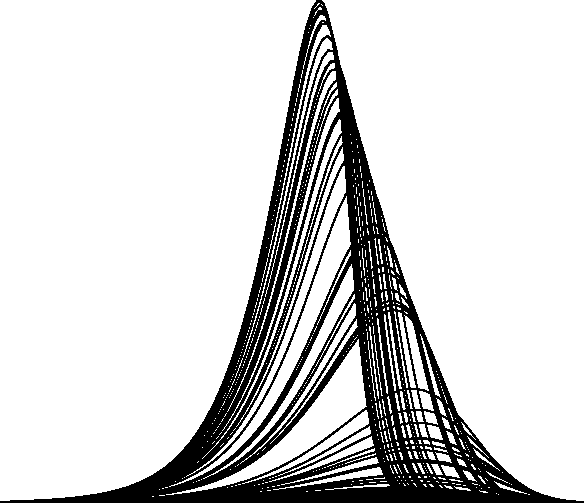
\includegraphics[width=0.9\paperwidth,height=0.85\paperheight]{files/possible.pdf}
  }%
}

% for placeholdezr text
\title{INTRODUCTION TO NUMERICAL SOLUTION OF FRACTIONAL SYSTEMS}
\author{David Plazas E.\\Mateo Restrepo S.\\Juan Sebastián Cárdenas-Rodríguez}

\begin{document}
\BgThispage
\maketitle
\thispagestyle{empty}

\newpage
\tableofcontents

\chapter{Fractional Calculus}

The idea behind fractional operators started when L'Hôpital asked Leibniz whether an extension to integer-order derivatives could be done, i.e. $d^\alpha y/dx^\alpha$ when $\alpha\notin\mathbb{N}$. At the time, the idea did not captivate enough attention; nowadays, multiple physical applications have been proposed, mostly as generalization of known systems \cite{deng2012numerical}. 

On the other hand, fractional derivatives have multiple definitions, depending on the author that studied them; for example Euler, Fourier, Abel, Liouville, Riemann, Letnikov, Grünwald, Caputo, Miller, etc \cite{dalir2010applications}. In this book, the Caputo-type fractional derivatives will be used since, as we will discuss further in this work, they satisfy an important property to simulate physical systems.

Some applications of fractional calculus (from \cite{dalir2010applications}):
\begin{multicols}{2}
\begin{itemize}
    \item \textit{The tautochrone problem} (Abel's approach) \cite{kisela2008fractional}.
    \item \textit{Electric transmission lines} (Heaviside) \cite{heaviside1899theory}.
    \item \textit{Ultrasonic wave propagation in human cancellous bone} (Sebaa \textit{et al.}) \cite{sebaa2006application}.
    \item \textit{Modeling of speech signals using fractional calculus} (Assaleh \& Ahmad) \cite{assaleh2007modeling}.
    \item \textit{Modeling the cardiac tissue electrode interface using fractional calculus} (Magin \& Ovadia) \cite{magin2006modeling}.
    \item \textit{Application of fractional calculus to the sound waves propagation in rigid porous materials} (Fellah \& Depollier) \cite{fellah2002application}.
    \item \textit{Using fractional calculus for lateral and longitudinal control of autonomous vehicles} (Su\'arez \textit{et al.}) \cite{suarez2003using}.
    \item \textit{Application of fractional calculus in the theory of viscoelasticity} (Soczkiewicz) \cite{soczkiewicz2002application}.
    \item \textit{Fractional differentiation for edge detection} (Mathieu \textit{et al.}) \cite{mathieu2003fractional}.
    \item \textit{Wave propagation in viscoelastic horns using a fractional calculus rheology model} (Marguiles) \cite{margulies2003wave}.
    \item \textit{Application of fractional calculus to fluid mechanics} (Kulish \& Lage) \cite{kulish2002application}.
\end{itemize}
\end{multicols}

It is considered that fractional derivatives have some advantages and disadvantages
\begin{multicols}{2}
    \textbf{Advantages}
    \begin{itemize}
        \item Generalization of ordinary derivatives.
        \item Nonlocal operators $\longrightarrow$ Memory and heritage.
        \item More accuracy and robustness.
        \item Unexplored areas and applications.
    \end{itemize}
    \columnbreak
    \textbf{Disadvantages}
    \begin{itemize}
        \item There are multiple fractional derivatives definitions.
        \item The derivatives are not always in terms of elementary functions.
        \item Some definitions require strong conditions on the functions to differentiate.
    \end{itemize}
    \end{multicols}

\section{Preliminaries}
\subsection{Gamma Function}\label{subsec:gamma}
While treating fractional derivatives, the following definition will come in handy. The Gamma Function is defined by the improper integral

\begin{equation}
    \Gamma(z) = \int_0^\infty t^{z-1}e^{-t}dt\quad \mathrm{Re}(z)>0
\end{equation}

This function has some special properties: $\Gamma(z+1)=z\Gamma(z)$ and $\Gamma(1/2)=\sqrt{\pi}$. In figure \ref{fig:gamma}, the curve for the gamma function is shown.

\begin{figure}[H]
    \centering
    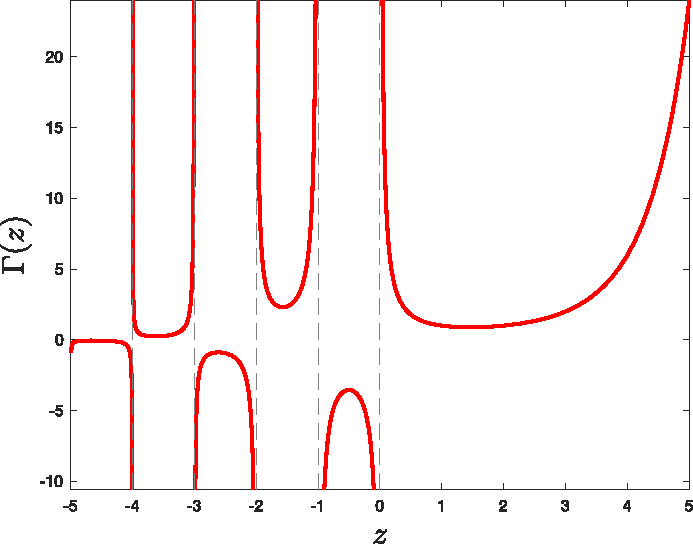
\includegraphics[scale=0.5]{files/gamma.pdf}
    \caption{The gamma function.}
    \label{fig:gamma}
\end{figure}

\subsection{Beta Function}
The Beta function is used for obtaining some important results in fractional calculus. This function is defined as

\begin{equation}
    B(z,w)=\int_0^1 t^{z-1}(1-t)^{w-1}dt\quad z,w>0
\end{equation}

The Beta function can be as well defined in terms of the Gamma function (section \ref{subsec:gamma})
\begin{equation}
    B(z,w)=\dfrac{\Gamma(z)\Gamma(w)}{\Gamma(z+w)}
\end{equation}
Note that $B(z,w)=B(w,z)$.

\subsection{Mittag-Leffler Function}
The Mittag-Leffler function is a special-complex function defined as
\begin{equation}
    E_{\alpha,\beta}(z)=\sum_{k=0}^{\infty}\dfrac{z^k}{\Gamma(\alpha k +\beta)} \quad z\in\mathbb{C}
\end{equation}

Where $\alpha,\,\beta\in\mathbb{R}$ and $\Gamma(\cdot)$ is the gamma function. 

\begin{figure}[H]
    \centering
    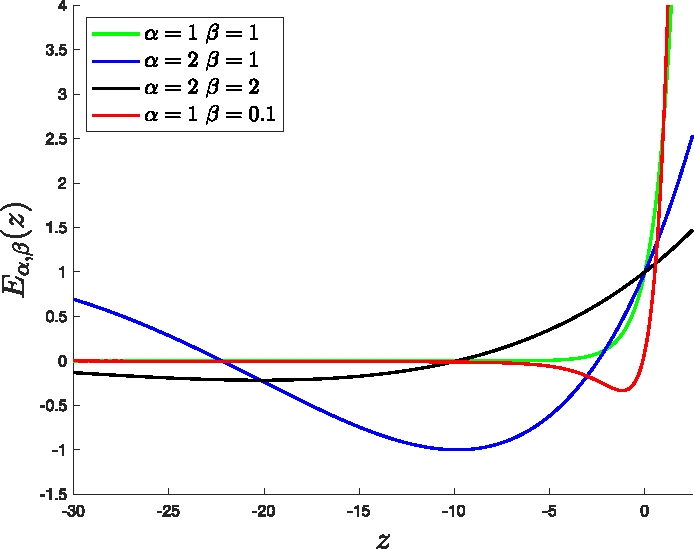
\includegraphics[scale=0.5]{files/mittag.pdf}
    \caption{Mittag-Leffler functions for some $\alpha$ and $\beta$.}
    \label{fig:mittag}
\end{figure}

\subsection{Riemann-Liouville Integral}\label{sec:RL}
The Riemann-Liouville integral of order $\alpha$ is defined as
\begin{equation}
    J^\alpha y(t) = \dfrac{1}{\Gamma(\alpha)}\int_{0}^{t}\dfrac{y(\lambda)}{(t-\lambda)^{1-\alpha}}d\lambda
\end{equation}

\begin{theorem}
Let $\alpha,\beta\in\mathbb{R}^+$, then
\begin{equation}
    J^\alpha J^\beta y(t) = J^{\alpha+\beta} y(t)
\end{equation}
\end{theorem}
\begin{proof}
\begin{align*}
    J^{\alpha}J^{\beta}y(t)&=\dfrac{1}{\Gamma(\alpha)} \int_0^t\dfrac{\left(J^{\beta}y(t)\right)(\lambda_1)}{(t-\lambda_1)^{1-\alpha}}d\lambda_1\\
    &=\dfrac{1}{\Gamma(\alpha)} \int_0^t\dfrac{1}{(t-\lambda_1)^{1-\alpha}\Gamma(\beta)}\int_0^{\lambda_1}\dfrac{y(\lambda_2)}{(\lambda_1-\lambda_2)^{1-\beta}}d\lambda_2d\lambda_1\\
    &=\dfrac{1}{\Gamma(\alpha)\Gamma(\beta)}\int_0^{t}\int_0^{\lambda_1}(t-\lambda_1^{\beta-1})(\lambda_1-\lambda_2)^{\alpha-1}y(\lambda_2)d\lambda_2d\lambda_1\\
    &=\dfrac{1}{\Gamma(\alpha)\Gamma(\beta)}\int_0^{t}\int_{\lambda_2}^t (t-\lambda_1^{\beta-1})(\lambda_1-\lambda_2)^{\alpha-1}y(\lambda_2)d\lambda_1d\lambda_2\\
    &=\dfrac{1}{\Gamma(\alpha)\Gamma(\beta)}\int_0^{t}y(\lambda_2)\int_{\lambda_2}^t(t-\lambda_1^{\beta-1})(\lambda_1-\lambda_2)^{\alpha-1}y(\lambda_2)d\lambda_1d\lambda_2\\
\end{align*}
Multiplying and dividing by $(t-\lambda_2)^{\alpha+\beta-2}$
\begin{align*}
    J^{\alpha}J^{\beta}y(t)&=\dfrac{1}{\Gamma(\alpha)\Gamma(\beta)}\int_0^{t}(t-\lambda_2)^{\alpha+\beta-2}y(t_2)\int_{\lambda_2}^{t}\left(\dfrac{t-\lambda_1}{t-\lambda_2}\right)^{\beta-1}\left(\dfrac{\lambda_1-\lambda_2}{t-\lambda_2}\right)^{\alpha-1}d\lambda_1d\lambda_2
\end{align*}
Let $u=\dfrac{\lambda_1-\lambda_2}{t-\lambda_2}\rightarrow du=\dfrac{d\lambda_1}{t-\lambda_2}$. Note that $1-u=\dfrac{t-\lambda_1}{t-\lambda_2}$
\begin{align*}
    J^{\alpha}J^{\beta}y(t)&=\dfrac{1}{\Gamma(\alpha)\Gamma(\beta)}\int_0^{t}(t-\lambda_2)^{\alpha+\beta-2}y(t_2)\int_0^1\dfrac{u^{\beta-1}(1-u)^{\alpha-1}}{t-\lambda_2}dud\lambda_2\\
    &=\dfrac{1}{\Gamma(\alpha)\Gamma(\beta)}\int_0^{t}(t-\lambda_2)^{\alpha+\beta-1}y(t_2)B(\beta,\alpha)d\lambda_2\\
    &=\dfrac{1}{\Gamma(\alpha+\beta)}\int_0^{t}(t-\lambda_2)^{\alpha+\beta-1}y(t_2)d\lambda_2=J^{\alpha+\beta}y(t)
\end{align*}
\end{proof}



\section{Caputo Fractional Derivative}

The $\alpha$-order Caputo derivative is defined as 
\begin{equation}
    \mathcal{D}_c^\alpha y(t) = J^{m-\alpha}y^{(m)}(t) = \dfrac{1}{\Gamma(m-\alpha)}\int_0^t \dfrac{y^{(m)}(\lambda)}{(t-\lambda)^{1-m+\alpha}}d\lambda
\end{equation}

Where $m = \ceil{\alpha}$. We assume $\alpha\geq0$. Note that some authors, e.g. \cite{kisela2008fractional}, treat $\alpha<0$ as a fractional integral. 

The main feature of the Caputo definition is that, when defining a fractional differential equation (FDE) involving this definition, they only require initial conditions for the derivatives of integer order, unlike Riemann-Liouville definition. This opens the FDEs to have an easier physical interpretation and modeling real systems.
\begin{exmp}
    Evaluate $\mathcal{D}_c^{0.5}\,t$
    \begin{align*}
      \mathcal{D}_c^{0.5}\,t &= \dfrac{1}{\Gamma(1-0.5)}\int_0^t \dfrac{d}{d\lambda}(\lambda)\cdot\dfrac{d\lambda}{(t-\lambda)^{1-0.5+1}}\\
      &= \dfrac{1}{\sqrt{\pi}}\int_0^t \dfrac{d\lambda}{(t-\lambda)^{1/2}}\quad\text{, let $u=t-\lambda$ $\rightarrow$ $du=-d\lambda$.}\\
      &= \dfrac{1}{\sqrt{\pi}}\int_0^t \dfrac{du}{u^{1/2}}\\
      &=2\sqrt{\dfrac{t}{\pi}}
    \end{align*}
\end{exmp}
    In order to illustrate the fractional derivative, we present the Caputo derivative of $y(t)=t$ for different orders in figure \ref{fig:t_derivative}. It can be proved that the Caputo-type derivative converges to the standard derivative for integer orders \cite{ishteva2005properties}, as depicted in this figure.
    
    \begin{figure}[H]
        \centering
        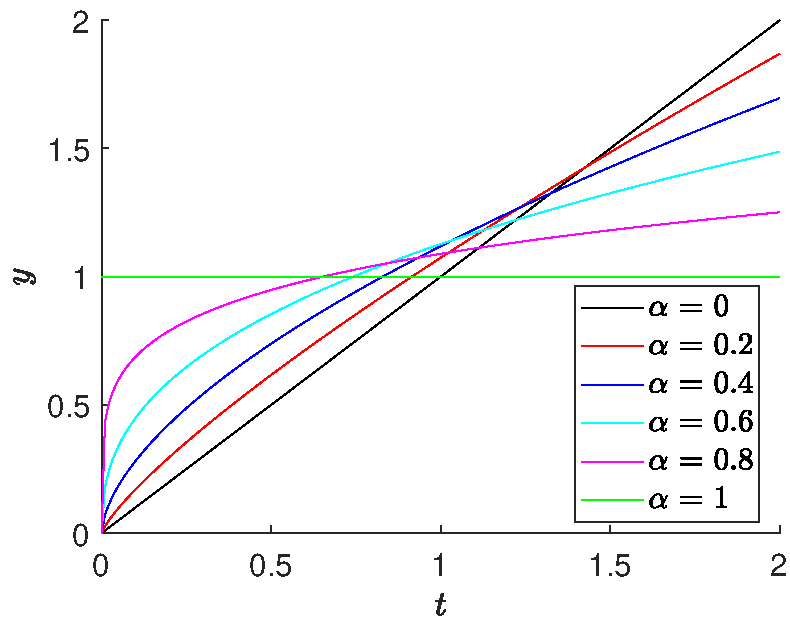
\includegraphics[scale=.5]{files/t_derivative.pdf}
        \caption{Fractional derivatives of $y(t)=t$ for different orders.}
        \label{fig:t_derivative}
    \end{figure}
    
    \begin{exmp}
        Evaluate $\mathcal{D}_c^\alpha\,t^r$
        \begin{align*}
        \mathcal{D}_c^\alpha\,t^r &= \dfrac{1}{\Gamma(m-\alpha)} \int_0^t \dfrac{d^m}{d\lambda^m}(\lambda^r)\cdot\dfrac{d\lambda}{(t-\lambda)^{1-m+\alpha}}\\
        & = \dfrac{1}{\Gamma(m-\alpha)}\int_0^t \dfrac{\Gamma(r+1)}{\Gamma(r-m+1)}\lambda^{r-m}\cdot\dfrac{d\lambda}{(t-\lambda)^{1-m+\alpha}}\\
        &= \dfrac{\Gamma(r+1)}{\Gamma(m-\alpha)\Gamma(r-m+1)}\int_0^t \lambda^{r-m}(t-\lambda)^{m-\alpha-1}d\lambda
    \end{align*}
    \end{exmp}
    Let $\lambda = u t$ $\rightarrow$ $d\lambda=tdu$. Note that $0\leq u\leq 1$.
    \begin{align*}
        \mathcal{D}_c^\alpha\,t^r &= \dfrac{\Gamma(r+1)}{\Gamma(m-\alpha)\Gamma(r-m+1)}\int_0^1 (u t)^{r-m}(t-u t)^{m-\alpha-1}tdu\\
        &=\dfrac{\Gamma(r+1)}{\Gamma(m-\alpha)\Gamma(r-m+1)}t^{r-\alpha}\int_0^1 u^{(r-m+1)-1}(1-u)^{(m-\alpha)-1}du\\
        &=\dfrac{\Gamma(r+1)}{\Gamma(m-\alpha)\Gamma(r-m+1)}t^{r-\alpha}\cdot B(r-m+1,m-\alpha)\\
        &=\dfrac{\Gamma(r+1)}{\Gamma(m-\alpha)\Gamma(r-m+1)}t^{r-\alpha}\cdot\dfrac{\Gamma(r-m+1)\Gamma(m-\alpha)}{\Gamma(r-\alpha+1)}\\
        &= \dfrac{\Gamma(r+1)}{\Gamma(r-\alpha+1)}t^{r-\alpha}\\
    \end{align*}
    
    \begin{theorem}\label{theo:leftinverse}
        $\mathcal{D}_c^\alpha$ is a left-inverse operator for $J^\alpha$.
    \end{theorem}
    \begin{proof}
        \begin{equation}
    \mathcal{D}_c^\alpha J^\alpha y(t) = J^{m-\alpha}\underset{\Delta}{\underbrace{\left(\dfrac{d^m}{dt^m}J^\alpha y(t)\right)}}
\end{equation}\label{eq:Jinverse}
Let us work on $\Delta$ first,

\begin{align*}
    \Delta&=\dfrac{d^m}{dt^m}\left[\dfrac{1}{\Gamma(\alpha)}\int_0^t\dfrac{y(\lambda_1)d\lambda_1}{(t-\lambda_1)^{1-\alpha}}\right]\\
    &= \dfrac{1}{\Gamma(\alpha)}\left[\dfrac{d^m}{dt^m}\int_0^t\dfrac{y(\lambda_1)d\lambda_1}{(t-\lambda_1)^{1-\alpha}}\right]\\
\end{align*}

Recall the Leibniz rule
\begin{equation}
    \dfrac{d}{dx}\int_{a(x)}^{b(x)}f(x,t)dt = f(x,b(x))\dfrac{db(x)}{dx}-f(x,a(x))\dfrac{da(x)}{dx}+\int_{a(x)}^{b(x)}\dfrac{\partial f(x,t)}{\partial x}dt
\end{equation}

Therefore,
\begin{align*}
    =\dfrac{d^{m-1}}{dt^{m-1}}\left[(t-t)^{\alpha-1}y(t) - 0 + \int_{0}^t \dfrac{(\alpha-1)y(\lambda_1)d\lambda_1}{(t-\lambda_1)^{2-\alpha}}\right]
\end{align*}

Applying this process recursively,
\begin{align*}
    =\dfrac{\Gamma(\alpha)}{\Gamma(\alpha-m)}\int_0^t\dfrac{y(\lambda_1)d\lambda_1}{(t-\lambda_1)^{1+m-\alpha}}
\end{align*}

Replacing in equation \eqref{eq:Jinverse},
\begin{align*}
    J^{m-\alpha}\left(\dfrac{d^m}{dt^m}J^\alpha y(t)\right)=&\dfrac{1}{\Gamma(\alpha-m)\Gamma{(m-\alpha)}}\int_0^t \dfrac{1}{(t-\lambda_2)^{1+\alpha-m}}\int_0^{\lambda_2} \dfrac{y(\lambda_1)d\lambda_1d\lambda_2}{(\lambda_2-\lambda_1)^{1-\alpha+m}}\\
    =& \dfrac{1}{\Gamma(\alpha-m)\Gamma{(m-\alpha)}}\int_0^t\int_0^{\lambda_2}  \dfrac{y(\lambda_1)d\lambda_1d\lambda_2}{(t-\lambda_2)^{1+\alpha-m}(\lambda_2-\lambda_1)^{1-\alpha+m}}\\
    =& \dfrac{1}{\Gamma(\alpha-m)\Gamma{(m-\alpha)}}\int_0^t\int_{\lambda_1}^{t}
    \dfrac{y(\lambda_1)d\lambda_2d\lambda_1}{(t-\lambda_2)^{1+\alpha-m}(\lambda_2-\lambda_1)^{1-\alpha+m}}\\
    =& \dfrac{1}{\Gamma(\alpha-m)\Gamma{(m-\alpha)}}\int_0^ty(\lambda_1)\int_{\lambda_1}^{t}
    \dfrac{d\lambda_2d\lambda_1}{(t-\lambda_2)^{1+\alpha-m}(\lambda_2-\lambda_1)^{1-\alpha+m}}
\end{align*}
Multiplying and dividing by $(t-\lambda_1)^{-2}$ yields

\begin{align*}
    J^{m-\alpha}\left(\dfrac{d^m}{dt^m}J^\alpha y(t)\right)=& \dfrac{1}{\Gamma(\alpha-m)\Gamma{(m-\alpha)}}\int_0^t(t-\lambda_1)^{-2}y(\lambda_1)\int_{\lambda_1}^{t} \psi(t,\lambda_1,\lambda_2,\alpha,m)d\lambda_2d\lambda_1
\end{align*}
where
\begin{equation*}
\psi(t,\lambda_1,\lambda_2,\alpha,m)=\left(\dfrac{t-\lambda_2}{t-\lambda_1}\right)^{m-\alpha-1}\left(\dfrac{\lambda_2-\lambda_1}{t-\lambda_1}\right)^{\alpha-1-m}
\end{equation*}


Let $u=\dfrac{\lambda_2-\lambda_1}{t-\lambda_1}\rightarrow du=\dfrac{d\lambda_2}{t-\lambda_1}$. Note that $1-u=\dfrac{t-\lambda_2}{t-\lambda_1}$, thus

\begin{align*}
    J^{m-\alpha}\left(\dfrac{d^m}{dt^m}J^\alpha y(t)\right)=& \dfrac{1}{\Gamma(\alpha-m)\Gamma{(m-\alpha)}}\int_0^t\dfrac{y(\lambda_1)}{(t-\lambda_1)}\int_{0}^{1}u^{\alpha-m-1}(1-u)^{m-\alpha-1}dud\lambda_1\\
    =& \dfrac{1}{\Gamma(\alpha-m)\Gamma{(m-\alpha)}}\int_0^t\dfrac{y(\lambda_1)}{(t-\lambda_1)} B(\alpha-m,m-\alpha)d\lambda_1\\
    =& \dfrac{1}{\Gamma(0)}\int_0^t\dfrac{y(\lambda_1)}{(t-\lambda_1)}d\lambda_1=J^0y(t)=y(t)
\end{align*}
    
        
    \end{proof}
    
    
    \begin{theorem}\label{theo:rightinverse}
        \begin{equation}
            J^\alpha \mathcal{D}_c^\alpha y(t) = y(t) - \sum_{r=0}^{m-1}\dfrac{y_{(r)}t^r}{r!}
        \end{equation}
    \end{theorem}
        \begin{proof}
        By definition of $\mathcal{D}_c^\alpha$ and properties of the Riemann-Liouville integral, we have\[ J^\alpha J^{m-\alpha}y^{(m)}(t)=J^my^{(m)}(t)\] Let us compute $J^my^{(m)}(t)$
        
        \begin{align*}
            J^my^{(m)}(t)=& \dfrac{1}{\Gamma(m)}\int_0^t \dfrac{y^{(m)}(\lambda)}{(t-\lambda)^{1-m}}d\lambda\\
            =& \dfrac{1}{\Gamma(m)}\int_0^t y^{(m)}(\lambda)(t-\lambda)^{m-1}d\lambda
        \end{align*}
        
        Using integration by parts (multiple times), $u=(t-\lambda)^{m-1}$ $\rightarrow$ $du=-(m-1)\cdot(t-\lambda)^{m-2}d\lambda$ and $dv=y^{(m)}(\lambda)d\lambda$ $\rightarrow$ $v = y^{(m-1)}(\lambda)$
        
        \begin{align*}
            J^my^{(m)}(t)=& \dfrac{1}{\Gamma(m)} \left[ y^{(m)}(\lambda) (t-\lambda)^{m-1}\Big|_0^t + (m-1)\int_0^t y^{(m-1)}(\lambda)(t-\lambda)^{m-2}d\lambda \right]\\
            &\hspace{4.4cm} \vdots\\
            &=\dfrac{1}{\Gamma(m)} \left[\sum_{k=0}^{m-1}\dfrac{(m-1)!}{(m-k-1)!}y^{(m-k-1)}(\lambda)(t-\lambda)^{m-k-1}\right]_0^t\\
            &=f(t)-\sum_{k=0}^{m-1}\dfrac{1}{(m-k-1)!}y^{(m-k-1)}(0)t^{m-k-1}
        \end{align*}
        
        Making $r=m-k-1$, we obtain the desired expression:
        \begin{equation}
            J^my^{(m)}(t)=y(t) - \sum_{r=0}^{m-1}\dfrac{y_{(r)}t^r}{r!}
        \end{equation}
        \end{proof}
        
    The following theorem will be useful for some results later in this manuscript. This theorem was extracted from \cite[p. 135]{diethelm2010analysis}.
        
    \subsection{Some Caputo Fractional Derivatives}
    The following formulas were extracted from \cite{ishteva2005properties}; please refer to this citation for more detailed information in this results.
    \begin{itemize}
        \item \textbf{Constant function}: $\forall \lambda\in\mathbb{R}$, \begin{equation}
            \mathcal{D}_c^\alpha \lambda = 0
        \end{equation}
        \item \textbf{Power function:} $\forall \lambda\in\mathbb{R}:\lambda>m-1$, $m = \ceil{\alpha}$
        \begin{equation}
            \mathcal{D} _ { c } ^ { a } t ^ { \lambda } = \dfrac { \Gamma ( \lambda + 1 ) } { \Gamma ( \lambda - \alpha + 1 ) } t ^ { \lambda - \alpha }
        \end{equation}
        \item \textbf{Exponential function:} $\forall\lambda\in\mathbb{R}$, with $m = \ceil{\alpha}$
        \begin{equation}
            \mathcal{D} _ {c } ^ { \alpha } e ^ { \lambda t } = \sum _ { k = 0 } ^ { \infty } \frac { \lambda ^ { k + m } t ^ { k + m - \alpha } } { \Gamma ( k + 1 + m - \alpha ) } = \lambda ^ { m } t ^ { m - \alpha } E _ { 1 , m - a + 1 } ( \lambda t )
        \end{equation}
    \item \textbf{Sine function: }$\forall\lambda\in\mathbb{R}$, with $m = \ceil{\alpha}$
        \begin{equation}
            \mathcal{D} _ { c } ^ { \alpha } \sin \lambda t = - \frac { 1 } { 2 } i ( i \lambda ) ^ { m } t ^ { m - \alpha } \left( E _ { 1 , m - \alpha + 1 } ( i \lambda t ) - ( - 1 ) ^ { m } E _ { 1 , m - \alpha + 1 } ( - i \lambda t ) \right)
        \end{equation}
        \item \textbf{Cosine function: }$\forall\lambda\in\mathbb{R}$, with $m = \ceil{\alpha}$
        \begin{equation}
            \mathcal{D} _ { c } ^ { \alpha } \cos \lambda t = \frac { 1 } { 2 } ( i \lambda ) ^ { m } t ^ { m - \alpha } \left( E _ { 1 , m - \alpha + 1 } ( i \lambda t ) + ( - 1 ) ^ { m } E _ { 1 , m - \alpha + 1 } ( - i \lambda t ) \right)
        \end{equation}
    \end{itemize}

\subsection{Physical Application: The Tautochrone Problem}
    
    We wish to find a curve such that, if an object starts on any point along this curve, the time that it requires to slide down to the origin is constant, moving without friction only by the force of gravity. It is important to remark that this problem does not necessarily require fractional derivatives, although the problem (proposed by Abel about three centuries ago \cite{kisela2008fractional}) was one of the first applications of fractional calculus.
    
    \begin{figure}[H]
        \centering
        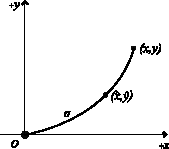
\includegraphics[scale=1.75]{files/taut.pdf}
        \caption{Tautochrone problem.}
        \label{fig:taut}
    \end{figure}
    
    Suppose we start somewhere in the $xy$ plane in a point $(x,y)$. Let $\sigma$ be the distance along the \textbf{curve} from the origin. Let us analyze the energy in a point $(\hat{x},\hat{y})$. 
    
    The energy conservation law states that $E_0 = E_f$, hence 
    
    \begin{equation}
        mgy = \dfrac{1}{2}mv^2 + mg\hat{y}
    \end{equation}
    
    Taking $v=\dfrac{d\sigma}{dt}$, we have
    \begin{align*}
        mgy &= \dfrac{1}{2}m\left(\dfrac{d\sigma}{dt}\right)^2 + mg\hat{y}\\
        \left(\dfrac{d\sigma}{dt}\right)^2 &= 2g(y-\hat{y})
    \end{align*}
    
    Note that $d\sigma/dt < 0$, since the object is approaching the origin. On the other hand, we assume $\sigma=\sigma(\hat{y}(t))$, therefore
    \begin{equation*}
        \dfrac{d\sigma}{dt}=\dfrac{d\sigma}{d\hat{y}}\cdot\dfrac{d\hat{y}}{dt}=\sigma'\dfrac{d\hat{y}}{dt}
    \end{equation*}
    
    Applying this, we have
    
    \begin{align*}
        \sigma'\dfrac{d\hat{y}}{dt} &= -\sqrt{2g(y-\hat{y})}\\
        \sigma'\dfrac{d\hat{y}}{\sqrt{y-\hat{y}}}&=\sqrt{2g}dt
    \end{align*}
    
    Integrating from $\hat{y}=0$ to $\hat{y}=y$ and $t$ from $t=0$ to $t=T$
    
    \begin{align*}
        \int_0^y \sigma'\dfrac{d\hat{y}}{\sqrt{y-\hat{y}}} &= \sqrt{2g}\int_0^Tdt\\
        \Gamma\left(1-\frac{1}{2}\right)\left[
        \dfrac{1}{\Gamma\left(1-\frac{1}{2}\right)}\int_0^y\sigma'\dfrac{d\hat{y}}{(y-\hat{y})^{1-1+\frac{1}{2}}}\right] &= \sqrt{2g}T
    \end{align*}
    Clearly, the inside of the left side of the equation is a Caputo-type fractional derivative. Hence,
    \begin{equation}
        \mathcal { D } _ { c } ^ { \frac { 1 } { 2 } } \sigma ( y ) = \frac { \sqrt { 2 g } } { \Gamma \left( \frac { 1 } { 2 } \right) } T
    \end{equation}
    
    This is a fractional differential equation for the function $\sigma(y)$, with initial condition $\sigma(0)=0$ since arc length at the origin is 0.
    Applying theorem \ref{theo:rightinverse}, we can apply the $\frac{1}{2}$-integral and obtain the solution. 
    \begin{align*}
        J^{\frac{1}{2}} \left[\mathcal { D } _ { c } ^ { \frac { 1 } { 2 } } \sigma ( y )\right] &= J^{\frac{1}{2}} \left[\frac { \sqrt { 2 g } } { \Gamma \left( \frac { 1 } { 2 } \right) } T \right] \\
        &= \dfrac{1}{\Gamma\left(\frac{1}{2}\right)}\int_0^y \dfrac{\frac { \sqrt { 2 g } } { \Gamma \left( \frac { 1 } { 2 } \right) } T}{(y-\lambda)^{1-\frac{1}{2}}}d\lambda\\
        &= \dfrac{\sqrt{2g}}{\left[\Gamma\left(\frac{1}{2}\right)\right]^2}T\int_0^y\dfrac{d\lambda}{(y-\lambda)^{\frac{1}{2}}}
    \end{align*}
    Let $u=y-\lambda\rightarrow du = -d\lambda$, then
    \begin{align*}
        J^{\frac{1}{2}} \left[\mathcal { D } _ { c } ^ { \frac { 1 } { 2 } } \sigma ( y )\right] &= \dfrac{\sqrt{2g}T}{\left[\Gamma\left(\frac{1}{2}\right)\right]^2}\int_0^y \dfrac{du}{u^{\frac{1}{2}}}\\
        &= \dfrac{2\sqrt{2g}T}{\left[\Gamma\left(\frac{1}{2}\right)\right]^2}u^{\frac{1}{2}}\bigg\rvert_0^y\\
        \sigma(y)&= \dfrac{2\sqrt{2g}T}{\pi}y^{\frac{1}{2}}
    \end{align*}
    Recall the formula for the distance along a curve
    \begin{equation}
        \dfrac{d\sigma}{dy}=\sqrt{1+\left(\dfrac{dx}{dy}\right)^2}
    \end{equation}
    
    Replacing, we have 
    
    \begin{equation}
        \dfrac{dx}{dy }=\sqrt{\dfrac{2gT^2}{\pi^2y}-1}
    \end{equation}\label{eq:tautfin}
    
    The solution to the ordinary differential equation is the solution to the Tautochrone problem. We will not prove the analytic solution. The solution to equation \ref{eq:tautfin} is given by the parametric expression
    \begin{align}
        x = \dfrac{gT^2}{\pi^2}[t+\sin(t)]\\
        y = \dfrac{gT^2}{\pi^2}[1-\cos(t)]
    \end{align}
    We could take $T=\dfrac{\pi}{\sqrt{2g}}$ in order to obtain $A=1$ and draw the Tautochrone easily:
    
    \begin{figure}[H]
        \centering
        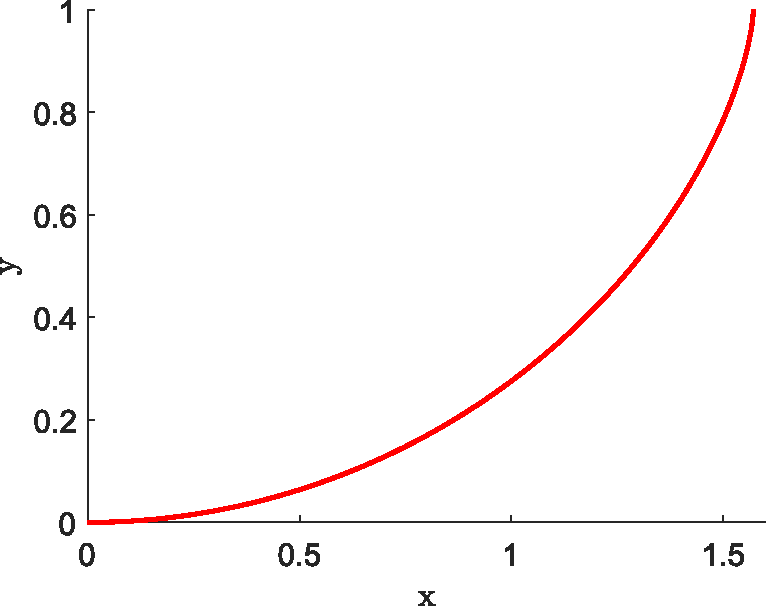
\includegraphics[scale=0.5]{files/tautochrone.pdf}
        \caption{Example of Tautochrone.}
    \end{figure}
    
    Which is an example of a Tautochrone: it does not matter the initial point along that curve, an object will always fall in the same time into the origin. It is important to mention that the tautochrone problem has a wide variety of procedures to be solved, but it is a clear example of fractional models in the real world.

\section{Real Phenomena with Fractional Models}
This section is intended to suggest the reader some evidence regarding the utility of fractional models in real world. This section is adapted from the work presented by Almeida \textit{et al.} in \cite{almeida2016modeling}.

\subsection{Population Growth}
In the paper, the authors consider the standard population growth approach (Malthusian Law). Let $P(t)$ be the population at an arbitrary time $t\geq0$, and $k$ a constant production rate, then 
\begin{equation}
    \begin{cases}
        P'(t)=kP(t)&\\
        P(0)=P_0&
    \end{cases}
\end{equation}
is the model of the population through time. The exact solution to this initial value problem can be found with straight-forward integration, yielding 
\begin{equation}
    P(t)=P_0e^{kt}, \quad t\geq0
\end{equation}
As the authors proposed, the idea is to replace the standard differential operator for fractional Caputo-type derivatives. Hence, the fractional approach to the population growth model is 
\begin{equation}
    \begin{cases}
        \mathcal{D}_c^\alpha P(t)=kP(t)&\\
        P(0)=P_0&
    \end{cases}
\end{equation}

\subsection{Blood Alcohol Level}



\section{Introduction}
In the 1920s, Charles Ponzi duped investors when he convinced them that he will return a 50\% revenue every 90 days; he was actually paying the old investors with the money given by the new ones. This is known as the Ponzi Scheme nowadays; since the virtual currencies lack of regulation and have enhanced privacy for trading, they can be and are being used by fraudsters to perpetrate their frauds in similar fashion \cite{ponzi}.

\noindent In 2017, the cryptocurrency company BitConnect launched its new coin BitConnect Coin (BCC, not to be confused with BitCoin Cash), which assured every user that whatever investment they made in their currency and made part of their loan and exchange platform (which allowed them to loan the company USD and Bitcoin to the company in favor of some interests) they will return up to 40\% of their initial investment every month. After using broad marketing strategies to avoid their investors to know about their fraudulent intentions and recollecting thousands of investments, they closed the loan and exchange platform; so, all the people who invested in the BCC lost all their money because of the 96\% drop in the price of the coin. Even the company promised to return some money for the people who got affected by given them the average of the price of the coin in the last 15 days but, given that BCC was at such a low price there were several financial lossess by the investors. In this day and age, there are new companies like XRPConnect, EthConnect, Bunny Token and NEOConnect that are replicating the schemes that BCC made without any type of regulation which, as what happened with BitConnect, can lead to disastrous results \cite{nextWeb}.

\noindent In this manner, cryptocurrencies can over-inflate their price by artificially manipulating the price by marketing it with unrealistic expectations so people start buying the coin and in some delay, selling it to other people to obtain profit through the Exchanges or the Peer to Peer system, who would put more coins in the market through mining. As they exploit the price and people invest more in the coin, they then can abuse this by incrementing by a big margin their Exchange rate or, on the other side, the company changes the coins it possesses for USD or another currency and, proceed to devaluate their coin so they do not have to pay people back. \cite{bcc11}.

\noindent On the other hand, price leveraging is not as hard in cryptocurrencies as other stocks that are available in the market. An article written in the Journal of Monetary Economics about the price manipulation in the bitcoin system, that the sudden spike in the price of bitcoin in 2013 happened due to suspicious activity in an exchanges called ``Mt.Gox Bitcoin Currency Exchange'', which 600000 BTC valued at 188 million USD were acquiered using bots, artificially inflating the price without any real substance; the article explains how this could have a massive effect in the growth rate of BTC in a positive manner, reaching a 4\% growth rate each day after \cite{PMitBE}.

\subsection{Problem of cryptocurrencies}
Taking account of all the above, the cryptocurrency system allows for people to abuse it in fraudulent ways to augment the growth rate of the price of that coin without any type of repercusion, due to the lack of goverment regulation. On the other hand, as an articles of forbes says, most of investors in this currencies like this investment because of the same lack of government involvement \cite{forbes}. In this manner, nowadays companies like Bunny Token, ETH Connect, XRPConnect and mire are expecting 1\% growth in their price daily without any type of proof or security for the investors without too much control because, of the lack of control they have, leading to a easier atmosphere to scam people.

\indent To conclude, it's important to notice that even if the problem and the variables have a very short span, there can be found a lot of documentation about them because they were one of the trending topics last year. Most people see Bitcoin and other cryptocurrencies as a safe economic investment and a way to make easy profit. Although we are not saying that is something that we should thrive to eliminate completely, it is important to examine how this system works and start to make policies that makes investing in this opportunity a safer place for the consumer and, stop catastrophes like BitConnect to don't ever happen again.




\section{Integer Case}


In this section, we will be treating the initial value problem (i.v.p.)
\begin{equation}\label{eq:iode}
\begin{cases}
    y'= f(t,y)&\\ y(0)=y_0\quad t\in[0,T]&
\end{cases}
\end{equation}
It is important to acknowledge that these numerical procedures can only treat first order ordinary differential equations. For solving higher order ordinary differential equations, the model has to be converted to an state-space representation (system of first order differential equations. In further sections, this methodology will be explained.

\subsection{Euler's Method}\label{sec:euler}
Euler's method \cite{euler} is the most basic procedure for solving ordinary differential equations. It takes advantage of the Taylor expansion of a function $f$, given by
\begin{equation}
y(t+h)=\sum_{n=0}^{\infty}\dfrac{y^{(n)}(t)}{n!}h^n=y(t)+hy'(t)+\dfrac{h^2}{2!}y''(t)+\dfrac{h^3}{3!}y'''(t)+\dots
\end{equation}
For $h\ll1$, we have $h^n\rightarrow0$ for $n\geq2$. Therefore,
\[y(t+h)\approx y(t)+hy'(t)=y(t)+hf(t,y(t))\]
\begin{equation}\label{eq:euler}
    y_{i+1}\approx y_i+hf(t_i,y_i)
\end{equation}


With expression \eqref{eq:euler}, a discrete approximation for the initial value problem \eqref{eq:iode} can be obtained, where $h$ is known as the step size for the algorithm. Note that this method only requires the previous approximation to calculate the next one; and, in order to calculate the first one, the initial conditions are applied. Remark: the Euler's method is a first-order numerical method since it only calculates the approximation for the next iteration. In the following section, we will explain how Euler's method works.

\subsubsection{Visualization}
\noindent Taking a closer look to Euler's method, it can be observed that equation \eqref{eq:iode} is an expression for the slope of the solution at any point $(t_i,y_i)$; therefore, if we were to calculate the next point $(t_{i+1},y_{i+1})$, we set $t_{i+1}=t_i+h$ and the $y_{i+1}$ is obtained by moving along the line with slope given by equation \eqref{eq:iode} throughout a time $h$. Formally this line would be $y=mt+b$ where $m=f(t_i,y_i)$ and $b=y_i$.

Let us present what we have already mentioned graphically:
\begin{figure}[H]
    \centering
    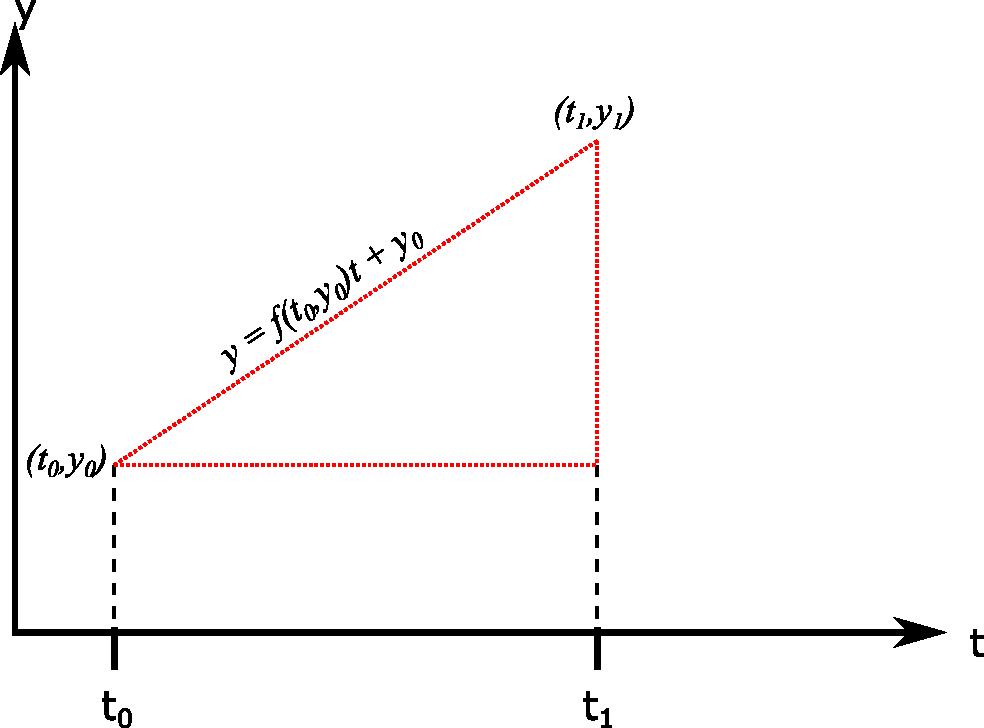
\includegraphics[scale=0.4]{files/graphicEuler.pdf}
    \caption{Visualization of Euler's method.}
    \label{fig:visualEuler}
\end{figure}

\subsubsection{Examples}
\begin{exmp} \label{ex:r_e}
Solve the following initial value problem using Euler's method \cite{exampleeuler}.
\begin{equation}
\begin{cases}
    y'+2y=2-e^{-4t}&\\ y(0)=1\quad t\in[0,2.5]&
\end{cases}
\end{equation}\label{eq:exeuler}
\end{exmp}
Throughout some calculus, the exact solution is
\begin{equation}
    y(t)=1+\dfrac{1}{2}e^{-4t}-\dfrac{1}{2}e^{-2t}
\end{equation}
For Euler's method, let us rewrite equation \eqref{eq:exeuler} as 
\begin{equation*}
    y'=2-e^{-4t}-2y
\end{equation*}
Now that we have the same form as the initial value problem \eqref{eq:iode}, let us apply Euler method with $f(t,y)=2-e^{-4t}-2y$ and $h=0.5$ for illustration purposes. In this case, we want to approximate the first five terms of the solution. Hence,
\begin{align*}
    y_0 =& y(0) = 1\\
    y_1 =& y_0+hf(t_0,y_0)= 1 + (0.5)\left[2-e^{-4\cdot0}-2(1)\right]=0.5\\
    y_2 =& y_1+hf(t_1,y_1) = 0.5 + (0.5)\left[2-e^{-4\cdot0.5}-2(0.5)\right]=0.9323\\
    &\qquad\qquad\qquad\qquad\qquad\qquad\vdots
\end{align*}
Following this procedure, one can obtain the results shown in table \ref{tab:euler}; this table shows the real value as well.

\begin{table}[H]
\centering
\begin{tabular}{cccc}
\hline
\textbf{i} & \textbf{t} & \textbf{Euler} & \textbf{Real} \\ \hline
0          & 0          & 1.0000         & 1.000         \\
1          & 0.5        & 0.5000         & 0.8837        \\
2          & 1          & 0.9323         & 0.9414        \\
3          & 1.5        & 0.9908         & 0.9763        \\
4          & 2          & 0.9987         & 0.9910        \\
5          & 2.5        & 0.9998         & 0.9966        \\ \hline
\end{tabular}
\caption{Comparison between the approximation and the real values.}
\label{tab:euler}
\end{table}
Notice that the approximation slightly differs from the real value, due to the large step size selected, though the general behavior of the solution is achieved; it is important to mention that the stationary state is successfully approximated since the differential equation describes an stable system.

In order to obtain better results, the step size can be reduced, leading to the following results, shown in figure (\ref{fig:taut}).

\begin{figure}[H]
    \centering
    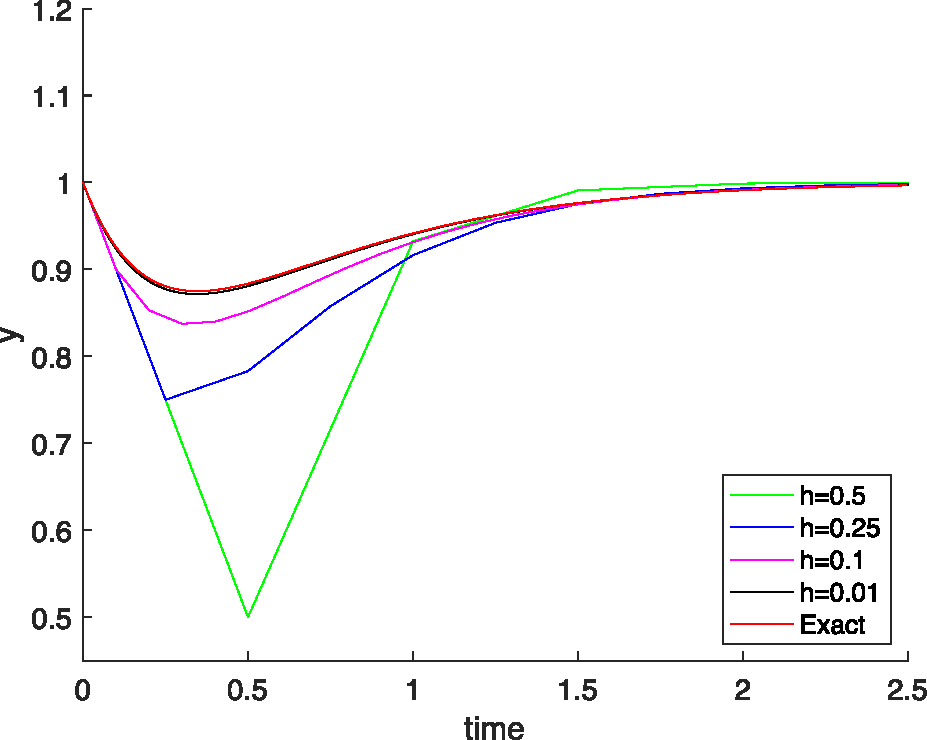
\includegraphics[scale=0.5]{files/exampleEuler.pdf}
    \caption{Results for smaller step sizes using Euler's method.}
    \label{fig:eulerHs}
\end{figure}

Notice that the approximation fits the exact curve as the step size is reduced. In order to illustrate the that Euler's method fails for certain type of differential equations, we shall present the following examples.

\begin{exmp}
Solve the following initial value problem using Euler's method \cite{exampleeuler}.
\begin{equation}
\begin{cases}
    y'-y=-\dfrac{1}{2}e^{\frac{t}{2}}\sin(5t)+5e^{\frac{t}{2}}\cos(5t)&\\ y(0)=0\quad t\in[0,7.5]&
\end{cases}
\end{equation}\label{eq:ex2euler}
\end{exmp}
Applying analytic procedures, the exact solution is given by
\begin{equation}
    y=e^{\frac{t}{2}}\sin(5t)
\end{equation}
In order to apply Euler's method, equation \eqref{eq:ex2euler} can be written as 
\begin{equation}
    y'= y-\dfrac{1}{2}e^{\frac{t}{2}}\sin(5t)+5e^{\frac{t}{2}}\cos(5t)
\end{equation}
As we have the same form as equation \eqref{eq:iode}, we may apply Euler's method with $f(t,y)=y-\dfrac{1}{2}e^{\frac{t}{2}}\sin(5t)+5e^{\frac{t}{2}}\cos(5t)$ and different step sizes to show the results. 

In table \ref{tab:ex2euler}, the results for different time steps and sampling for $t=1,...,7$, and in figure \ref{fig:ex2euler}.

\begin{table}[H]
\centering
\begin{tabular}{cccccc}
\hline
\textbf{Time}         & \textbf{\boldmath$h=0.5$} & \textbf{\boldmath$h=0.25$} & \textbf{\boldmath$h=0.1$} & \textbf{\boldmath$h=0.01$} & \textbf{Exact} \\ \hline
\boldmath{$t=0$} & 0&0&0&0&0\\
\boldmath{$t=1$} & 2.5000                    & 0.9615                     & -0.8028                   & -1.5278                    & -1.5810        \\
\boldmath{$t=2$} & 3.0437                    & 4.4541                     & 1.7565                    & -1.1177                    & -1.4788        \\
\boldmath{$t=3$} & 3.5231                    & 7.8287                     & 7.5072                    & 3.5863                     & 2.9144         \\
\boldmath{$t=4$} & 11.8335                   & 10.5377                    & 11.7976                   & 7.6874                     & 6.7458         \\
\boldmath{$t=5$} & 39.3181                   & 25.9843                    & 15.3996                   & 0.9441                     & -1.6124        \\
\boldmath{$t=6$} & 89.7192                   & 86.9894                    & 46.5853                   & -10.5407                   & -19.8451       \\
\boldmath{$t=7$} & 168.5382                  & 233.7051                   & 168.3623                  & 13.1961                    & -14.1795       \\ \hline
\end{tabular}
\caption{Numerical results using Euler's method and different step sizes.}
\label{tab:ex2euler}
\end{table}

\begin{figure}[H]
    \centering
    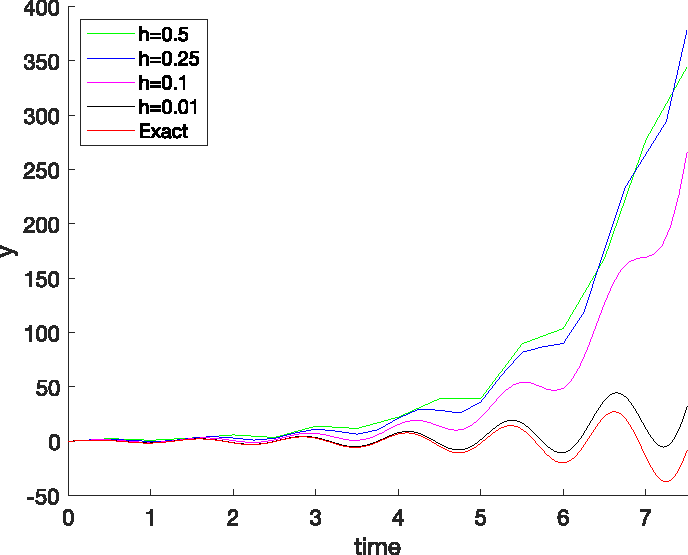
\includegraphics[scale=0.5]{files/example2Euler.pdf}
    \caption{Plots for the Euler's numerical approach with different time steps.}
    \label{fig:ex2euler}
\end{figure}

\begin{exmp}
Solve the following initial value problem using Euler's method.
\begin{equation}
\begin{cases}
    y' = 10e^{-\frac{(t-2)^2}{2}}\left(10\cos(10t)-(t-2)\sin(10t)\right)&\\ y(0) = 0 \quad t\in[0,7.5]&
\end{cases}
\end{equation}
\end{exmp}

The exact solution to this differential equation can be easily obtained and is given by

\begin{equation}
    y(t) = 10e^{-\frac{(t-2)^2}{2}}\sin(10t)
\end{equation}

As the previous examples, table \ref{tab:ex3euler} and figure \ref{fig:ex3euler} show the numeric solution using different time steps.

\begin{table}[H]
\centering
\begin{tabular}{cccccc}
\hline
\textbf{Time}           & \textbf{\boldmath$h=0.5$} & \textbf{\boldmath$t=0.25$} & \textbf{\boldmath$t=0.1$} & \textbf{\boldmath$t=0.01$} & \textbf{Exact} \\ \hline
\textbf{\boldmath$t=0$} & 0                    & 0                     & 0                    & 0                    & 0        \\
\textbf{\boldmath$t=1$} & 6.7668                    & 0.7530                     & 4.9597                    & -2.3979                    & -3.2997        \\
\textbf{\boldmath$t=2$} & -18.0595                  & -4.7931                    & -2.9158                   & 8.4869                     & 9.1295         \\
\textbf{\boldmath$t=3$} & -29.7418                  & 11.2838                    & -1.0473                   & -6.0916                    & -5.9927        \\
\textbf{\boldmath$t=4$} & 21.9611                   & -2.0837                    & 2.0016                    & 1.2339                     & 1.0084         \\
\textbf{\boldmath$t=5$} & 2.8130                    & 1.6074                     & 0.4535                    & 0.0203                     & -0.0291        \\
\textbf{\boldmath$t=6$} & 4.0794                    & 1.3343                     & 0.6358                    & 0.0666                     & -0.0010        \\
\textbf{\boldmath$t=7$} & 4.1062                    & 1.3357                     & 0.6300                    & 0.0672                     & 0.0000         \\ \hline
\end{tabular}
\caption{Numerical results using Euler's method for different step sizes.}
\label{tab:ex3euler}
\end{table}

\begin{figure}[H]
    \centering
    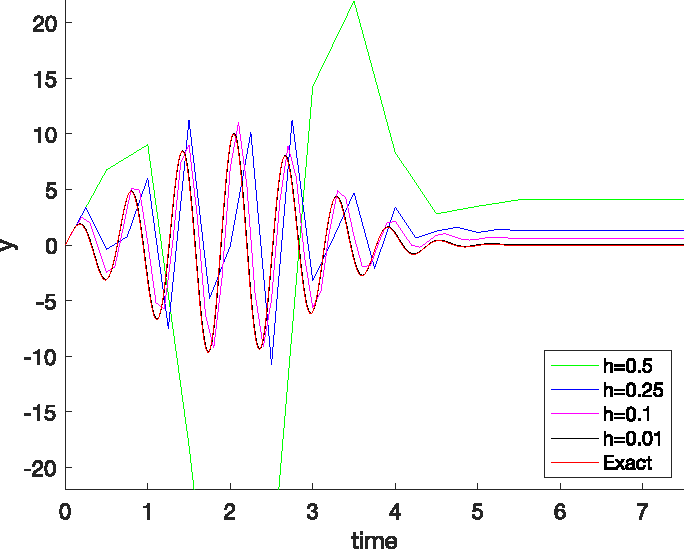
\includegraphics[scale=0.5]{files/example3Euler.pdf}
    \caption{Plots for numerical approach.}
    \label{fig:ex3euler}
\end{figure}

Notice that this differential equation describes an stable system, yet it does not fit the exact solution in stationary state; even with $h=0.1$, the numeric approximation does not stabilizes in the same value.

The previous two examples shows that Euler's method fails for functions that change rapidly and the approximation starts to separate from the exact solution. In order to obtain more exact approximations, we shall present the following numeric method.

\subsection{Fourth-Order Runge-Kutta Method}\label{sec:rk4}
The Runge-Kutta methods can be understood as an improvement of Euler's method. The most used order for Runge-Kutta methods is four, since for lower orders, the method is not accurate enough, and for higher orders, the method does not provide significant improvements in the approximations \cite{mathews2004numerical}.

The fourth-order Runge-Kutta (RK4) method is given by
\begin{equation}
    y _ { i + 1 } = y _ { i } + h\left(\dfrac{k_1+2k_2+2k_3+k_4}{6}\right)
\end{equation}
where 
\begin{equation*}
    \begin{array} { l } { k _ { 1 } = f \left( t _ { i } , y _ { i } \right) } \\
    { k _ { 2 } = f \left( t _ { i } + h / 2 , y _ { i } + h k _ { 1 } / 2 \right) } \\
    { k _ { 3 } = f \left( t _ { i } + h / 2 , y _ { i } + h k _ { 2 } / 2 \right) } \\ 
    { k _ { 4 } = f \left( t _ { i } + h , y _ { i } + h k _ { 3 } \right) } \end{array}
\end{equation*}

\subsubsection{Visualization}
This section is inspired and adapted on the explanation presented in \cite{vis_rk4}. Figure \ref{fig:RK4Visual} shows how RK4 works. It calculates four different slopes based on the previous one and then it takes the average of this slopes for a better accuracy. 

The method takes the slope at time $t=t_0$, for example, and then it makes an approximation just as Euler's method ($k_1$) until $t_1$, then it looks for the slope ($k_2$) in half that time through the same $y$ approximation as $k_1$; then, it looks for the half the change of $y$ then looks for the slope ($k_3)$ in the same time with this new $y$ value. Finally, it repeats this procedure in order to find the last slope ($k_4$).

Notice that this method includes the rate of change of the function between the time steps and after it, in order to calculate a more accurate slope and use it for the new approximation.

\begin{figure}[H]
    \centering
    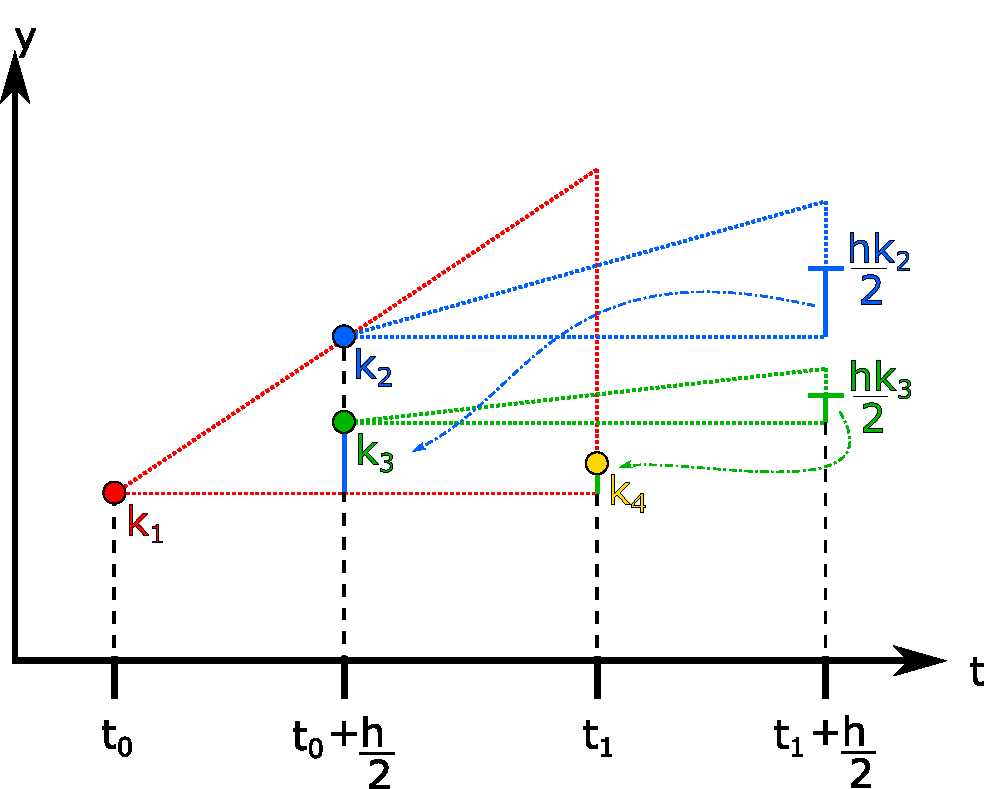
\includegraphics[scale=0.4]{files/sv.pdf}
    \caption{RK4 visualization.}
    \label{fig:RK4Visual}
\end{figure}


\begin{exmp}
Solve the following initial value problem using RK4 method \cite{exampleeuler}.
\begin{equation}
\begin{cases}
    y'+2y=2-e^{-4t}&\\ y(0)=1\quad t\in[0,2.5]& 
\end{cases}
\end{equation}
\end{exmp}
Notice that is the same  problem as the example \ref{ex:r_e}, where is shown the exact solution.
\begin{figure}[H]
    \centering
    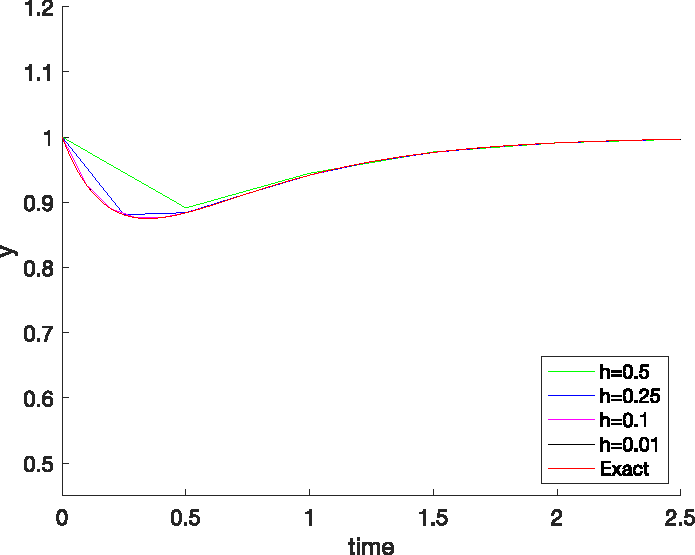
\includegraphics[scale=0.5]{files/exampleKutta.pdf}
    \caption{Results for smaller step sizes using RK4.}
    \label{fig:exkutta}
\end{figure}

In order to compare with the results obtained in section \ref{sec:euler}, let us use the same example.
\begin{exmp}
Solve the following initial value problem using RK4 method \cite{exampleeuler}.
\begin{equation}
\begin{cases}
    y'-y=-\dfrac{1}{2}e^{\frac{t}{2}}\sin(5t)+5e^{\frac{t}{2}}\cos(5t)&\\y(0)=0\quad t\in[0,7.5]&
    \end{cases}
\end{equation}\label{eq:ex2kutta}
\end{exmp}

\begin{table}[H]
\centering
\begin{tabular}{cccccc}
\hline
\textbf{Time}           & \textbf{\boldmath$h=0.5$} & \textbf{\boldmath$h=0.25$} & \textbf{\boldmath$h=0.1$} & \textbf{\boldmath$h=0.01$} & \textbf{Exact} \\ \hline
\textbf{\boldmath$t=1$} & 0.7628         & -0.8331         & -1.5331         & -1.5944          & -1.5810        \\
\textbf{\boldmath$t=2$} & 1.9905          & 1.4977           & -0.1943        & -1.3561          & -1.4788        \\
\textbf{\boldmath$t=3$} & -0.2875        & 3.6613           & 3.9855          & 3.0655           & 2.9144         \\
\textbf{\boldmath$t=4$} & -5.885         & -0.6581         & 4.2559          & 6.5538           & 6.7458         \\
\textbf{\boldmath$t=5$} & -5.2832         & -10.5996          & -6.8537         & -2.2028          & -1.6124        \\
\textbf{\boldmath$t=6$} & 9.5365          & -8.2108          & -17.9817         & -19.8755          & -19.8451       \\
\textbf{\boldmath$t=7$} & 19.1492          & 20.9004           & 1.8049          & -12.6028          & -14.1795       \\ \hline
\end{tabular}
\caption{Numerical results using RK4 method and different step sizes.}
\label{tab:ex2kutta}
\end{table}

\begin{figure}[H]
    \centering
    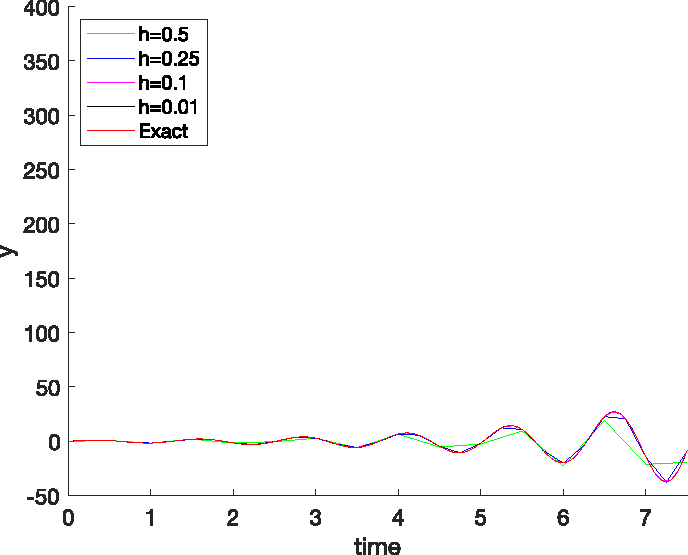
\includegraphics[scale=0.5]{files/example2Kutta.pdf}
    \caption{Results for smaller step sizes using RK4.}
    \label{fig:ex2kutta}
\end{figure}

\begin{exmp}
Solve the following initial value problem using RK4 method.
\begin{equation}
\begin{cases}
    y' = 10e^{-\frac{(t-2)^2}{2}}\left(10\cos(10t)-(t-2)\sin(10t)\right) &\\ y(0) = 0\quad t\in[0,7.5]&
\end{cases}
\end{equation}
\end{exmp}
As it was shown in previous sections, the exact solution is given by
\begin{equation}
    y(t) = 10e^{-\frac{(t-2)^2}{2}}\sin(10t)
\end{equation}


As the previous examples, table \ref{tab:ex3euler} and figure \ref{fig:ex3euler} show the numeric solution using different time steps.

\begin{table}[H]
\centering
\begin{tabular}{cccccc}
\hline
\textbf{Time}                          & \textbf{\boldmath$h=0.5$} & \textbf{\boldmath$h=0.25$} & \textbf{\boldmath$h=0.1$} & \textbf{\boldmath$h=0.01$} & \textbf{Exact} \\ \hline
\textbf{\boldmath$t=1$} & -3.5142                                  & 4.3668                                    & 2.2525                                   & -2.7473                                   & -3.2997        \\
\textbf{\boldmath$t=2$} & 14.5445                                  & -9.6097                                   & 1.4921                                   & 8.6760                                    & 9.1295         \\
\textbf{\boldmath$t=3$} & 1.8168                                   & 5.3571                                    & -4.4282                                  & -6.1167                                   & -5.9927        \\
\textbf{\boldmath$t=4$} & -4.4131                                  & -0.3869                                   & 1.5862                                   & 1.1155                                    & 1.0084         \\
\textbf{\boldmath$t=5$} & -0.2656                                  & -0.0688                                   & -0.1419                                  & -0.0409                                   & -0.0291        \\
\textbf{\boldmath$t=6$} & -0.7289                                  & 0.0268                                    & 0.0036                                   & -0.0007                                   & -0.0010        \\
\textbf{\boldmath$t=7$} & -0.7146                                  & 0.0194                                    & 0.0004                                   & 0.0000                                    & 0.0000         \\ \hline
\end{tabular}
\caption{Numerical results using RK4 method and different step sizes.}
\label{tab:ex3kutta}
\end{table}

\begin{figure}[H]
    \centering
    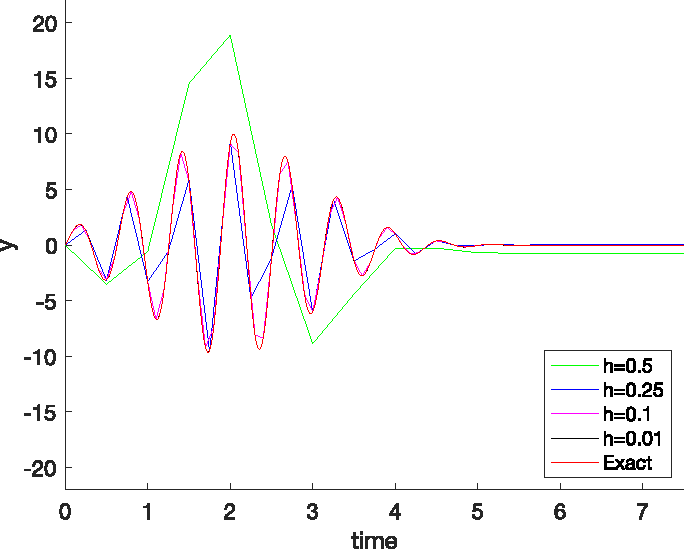
\includegraphics[scale=0.5]{files/example3Kutta.pdf}
    \caption{Plots for numerical approach.}
    \label{fig:ex3kutta}
\end{figure}

Notice than RK4 gives a significant improvement over the results obtained using Euler's method. Even for relatively large step sizes, the numeric approximation is bounded by the exact solution, and they stabilize closer to the exact solution, unlike Euler's method.

\section{Systems of Differential Equations}
When studying physical systems, higher order differential equations often arise, therefore a procedure to work on these models has to be presented. Another important reason to present the following methodology is that the numerical algorithms presented require the form of equation \eqref{eq:iode}, i.e. individual first order differential equations.

\subsection{Phase Variables}
The following procedure was obtained from \cite{rowell2002state} and \cite{antsaklis2006linear}. Suppose you have a system described by
\begin{equation}\label{eq:generalDiff}
\begin{cases}
    y^{(n)}(t)=f\left(y^{(n-1)},...,y'',y',y,t\right) &\\ y(0)=y_0,\,\dots,\,y^{(n - 1)}(0)= y_{(n - 1)}\quad t\in[0,T]&
\end{cases}
\end{equation}

and a solution is desired in an interval $[0,T]$. In order to convert this system into a system of first order differential equations, let us make the substitution in the phase variables, which allow us to represent the original system \eqref{eq:generalDiff} as follows
\begin{equation}
    \begin{cases}
        x_1 = y&\\
        x_2 = y'&\\
        \qquad\vdots&\\
        x_n = y^{(n-1)}&
    \end{cases}\longrightarrow
     \begin{cases}
        x'_1=x_2&\\
        x'_2=x_3&\\
        \qquad\vdots&\\
        x'_{n-1}=x_n&\\
        x'_n=f\left(x_n,x_{n-1},...,x_2,x_1,t\right)
    \end{cases}
\end{equation}
\begin{equation*}
    x_1(0)=y_0,\dots,\,x_{n - 1}(0)= y_{(n - 1)}
\end{equation*}

This system can be synthesized as 
\begin{equation}\label{eq:syn_sys_odes}
\begin{cases}
    \mathbf{x}'=F(\mathbf{x},t) &\\ \mathbf{x}(0) = \mathbf{x}_0\quad t\in[0,T]&
\end{cases}
\end{equation}
where $\mathbf{x}=[x_1\,\,x_2\,\,...\,\,x_n]^T$ is the state vector. Now we have obtained a set of $n$ first-order ordinary differential equations. In the following section, we will present how to work on these systems using the already presented methods.

\subsection{Numeric Simulation}
    \subsubsection{Euler}
    If it is wanted to simulate a system of first order differential equations through Euler's method, the following procedure is based on the original from section \ref{sec:euler} but with a slight twist: vectors instead of scalars.

    Let \[\mathbf{x}(j)=\left[x_1(j)\,\,x_2(j)\,\,\dots\,\, x_n(j)\right]^T\]
    be values of the $n$ variables of the system of $n$ differential equations at the iteration $j$. The iterative process to obtain the approximated solution is
    \begin{equation}
        \mathbf{x}(j+1)= \mathbf{x}(j)+hf(t_j,\mathbf{x})
    \end{equation}
    
    
    \subsubsection{Fourth-order Runge-Kutta}
    In order to simulate a system of differential equations with RK4, we use the same procedure described in section \ref{sec:rk4}, but treating the variable as a vector of variables. For a system of $n$, the recurrence formula for RK4 method will be
    \begin{equation}
        \mathbf{x}\left(j+1\right) = \mathbf{x}(j) + \dfrac{h}{6}\left(\mathbf{k}_1 + 2\mathbf{k}_2 + 2\mathbf{k}_3 + \mathbf{k}_4\right)
    \end{equation}
    Where: \[\mathbf{x}(j)=\left[x_1(j)\,\,x_2(j)\,\,\dots\,\, x_n(j)\right]^T\,\,\mathbf{k}_i=\left[k_{ix_1}\,\, k_{ix_2}\,\,\dots\,\, k_{ix_n}\right]^T\quad i=1,\,\dots,\,4\]
    And $k_{1x_k}$, $k_{2x_k}$, $k_{3x_k}$ and $k_{4x_k}$ will be defined exactly as they have been already shown in section \ref{sec:rk4}, but for each variable $x_k$. It is important to note that the simulation has to be performed sequentially, that is, it is necessary to calculate the whole state vector $\mathbf{x}$ at a time $t$ in order to calculate the next state vector at a time $t+1$.

    
    \begin{exmp} Higher Order ODEs: Consider the Duffing oscillator
    \begin{equation}
        y''+\delta y'+\alpha y+\beta y^{3}=\gamma \cos (\omega t)
    \end{equation}
    which has a wide variety of real applications in physical systems (see \cite{Korsch2008}). The equivalent system of first order ODEs is
    
    
    \begin{equation}
        \begin{cases}
        x_1 = y&\\
        x_2 = y'&\\
    \end{cases}\longrightarrow
    \begin{cases}
        x_1'=x_2&\\
        x_2'=-\delta x_2-\alpha x_1-\beta x_1^3 + \gamma\cos(\omega t)
    \end{cases}
    \end{equation}
    \end{exmp}
    
    Now we have a system of first order ODEs just as \ref{eq:syn_sys_odes}; now, Euler's or RK4 methods can be applied. The following simulation was performed using RK4 for $T=200s$ with $h=0.01$ with parameters $\delta=0.3$, $\alpha =-1$, $\beta=1$,$\gamma=0.37$, $\omega =1.2$ and initial conditions $x_1(0)=1$,  $x_2(0)=0$. The results are presented in figure \ref{fig:duffing}.
    
    \begin{figure}[H]
    \centering
    \begin{subfigure}[ht]{0.45\textwidth}
    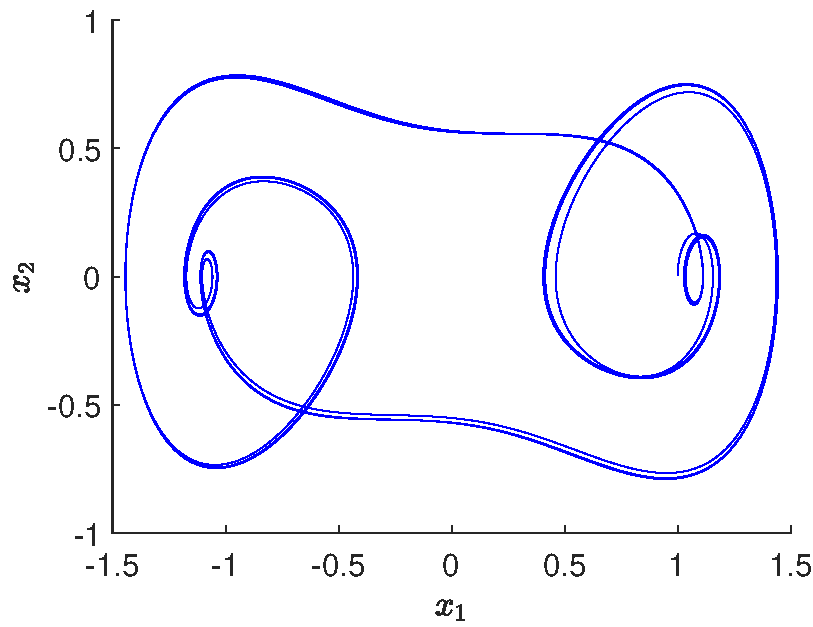
\includegraphics[scale=0.38]{files/duffing_phase.pdf}
    \end{subfigure}
    \begin{subfigure}[ht]{0.45\textwidth}
    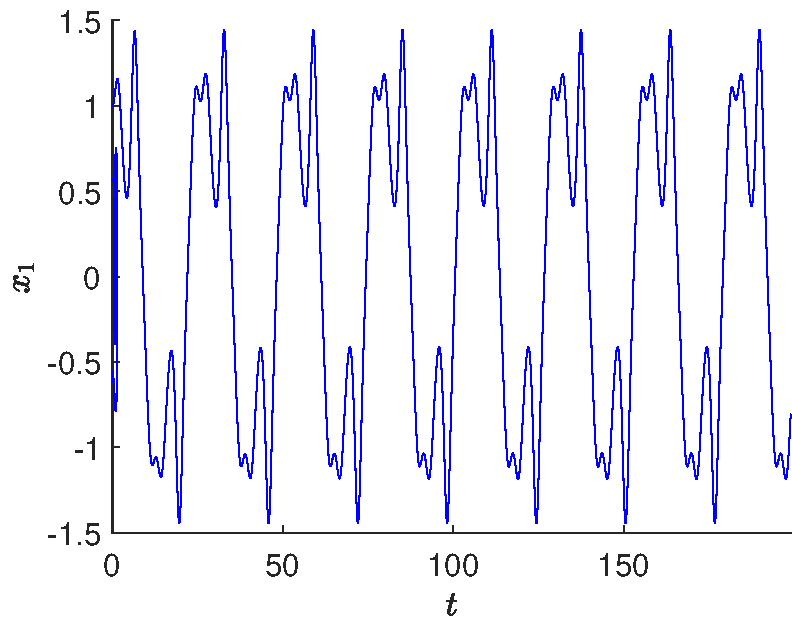
\includegraphics[scale=0.38]{files/duffing_time.pdf}
    \end{subfigure}
    \caption{Duffing oscillator simulation.}
    \label{fig:duffing}
    \end{figure}
    
    Although presented algorithms can be applied directly to systems of ODEs, let us show an example using RK4:
\begin{exmp} System of First Order ODEs:
    The Lotka-Volterra equations (predator-prey model) is a system of ODEs as follows:
\begin{equation}
    \begin{cases}{y_1'=\alpha y_1-\beta y_1 y_2}& \\ {y_2'=\delta y_1 y_2-\gamma y_2}&\end{cases}
\end{equation}
where $y_1$ represents the number of preys and $y_2$ is the amount of predators.

\begin{figure}[H]
    \centering
    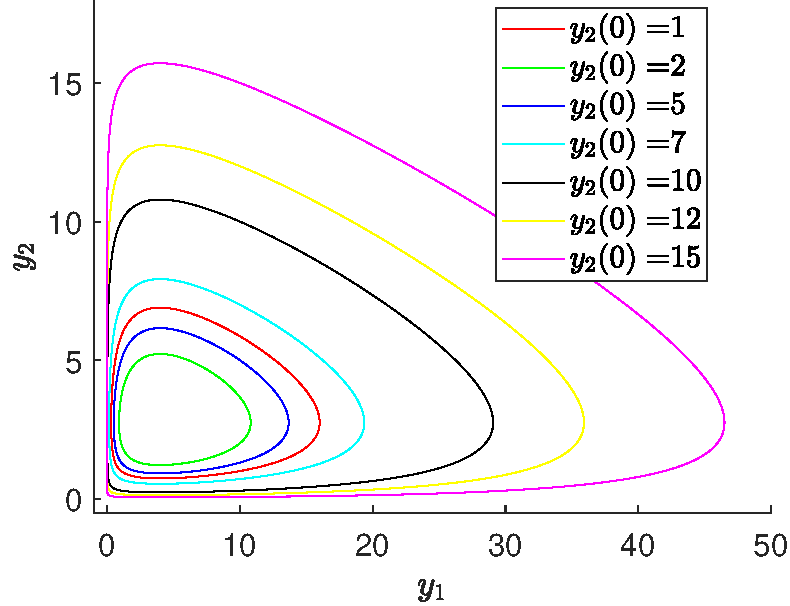
\includegraphics[scale=0.4]{files/Prey.pdf}
    \caption{Phase portrait of Lotka-Volterra equations.}
    \label{fig:lotka}
\end{figure}
\end{exmp}


\section{Fractional Differential Equations}

\subsection{Adams-Bashforth-Moulton Predictor-Corrector Algorithm}\label{sec:ABM}
The Adams-Bashforth-Moulton Predictor-Corrector method (ABM method), first proposed by Diethelm \textit{et al.} in \cite{diethelm2002predictor}, is a numerical algorithm to solve a fractional differential equation (FDE) in the form:

\begin{equation}\label{eq:frac_dif}
\begin{cases}
     \mathcal { D } _ { c } ^ { \alpha }y(t) = f(t,y)&\\ y(0)=y_0,\,\dots,y^{(\ceil{\alpha} - 1)}(0)= y_{(\ceil{\alpha} - 1)}\quad t\in[0,T]&
\end{cases}
\end{equation}

Applying the theorem \ref{theo:rightinverse} to \ref{eq:frac_dif} we get the following equation:
\begin{equation*}
    y(t)=\sum _{ k=0 }^{ m-1 }{ { y }_{ (k) }\frac { { x }^{ k } }{ k! }  } +\frac { 1 }{ \Gamma (\alpha ) } \int _{ 0 }^{ t }{ { (t-\lambda ) }^{ \alpha -1 }f(\lambda ,y(\lambda ))d\lambda  } 
\end{equation*}

Then, as explained in \cite{diethelm2002predictor}, the integral is approximated by quadrature theory. With this approximation, it is obtained that:

\begin{equation}
    \begin{aligned} y _ { h } \left( t _ { n + 1 } \right) = & \sum _ { k = 0 } ^ { [ \alpha ] - 1 } \frac { t _ { n + 1 } ^ { k } } { k ! } y _ { ( k ) } + \frac { h ^ { \alpha } } { \Gamma ( \alpha + 2 ) } f \left( t _ { n + 1 } , y _ { h } ^ { \mathrm { p } } \left( t _ { n + 1 } \right) \right) \\ & + \frac { h ^ { \alpha } } { \Gamma ( \alpha + 2 ) } \sum _ { j = 0 } ^ { n } a _ { j , n + 1 } f \left( t _ { j } , y _ { h } \left( t _ { j } \right) \right) \end{aligned}
\end{equation}

With:
\begin{equation*}
    a _ { j , n + 1 } = \left\{ \begin{array} { l l } { n ^ { \alpha + 1 } - ( n - \alpha ) ( n + 1 ) ^ { \alpha } , } & { \text { if } j = 0 } \\ { ( n - j + 2 ) ^ { \alpha + 1 } + ( n - j ) ^ { \alpha + 1 } - 2 ( n - j + 1 ) ^ { \alpha + 1 } , } & { \text { if } 1 \leq j \leq n } \\ { 1 , } & { \text { if } j = n + 1 } \end{array} \right.
\end{equation*}

And $y _ { h } ^ { \mathrm { p } } \left( t _ { n + 1 } \right)$ being a predicted value for the variable. To find this prediction, instead of approximating the integral by quadrature theory the product rectangle rule is used. Therefore, it is found that:

\begin{equation*}
    y _ { h } ^ { \mathrm { P } } \left( t _ { n + 1 } \right) = \sum _ { k = 0 } ^ { \lceil \alpha ] - 1 } \frac { t _ { n + 1 } ^ { k } } { k ! } y _ { ( k ) } + \frac { 1 } { \Gamma ( \alpha ) } \sum _ { j = 0 } ^ { n } b _ { j , n + 1 } f \left( t _ { j } , y _ { h } \left( t _ { j } \right) \right)
\end{equation*}

With:
\begin{equation*}
    b _ { j , n + 1 } = \frac { h ^ { \alpha } } { \alpha } \left( ( n + 1 - j ) ^ { \alpha } - ( n - j ) ^ { \alpha } \right)
\end{equation*}

There are some important aspects to notice about this method. First of all, for every iteration it needs every iteration prior because fractional derivatives have memory; but, this makes the algorithm to have a worst algorithmic complexity as the integer case (improvements for this will be discussed in chapter \ref{chap:modif}). Lastly, it is seen that a predicted value is necessary for calculating every iteration so, why don't use this predicted value instead as the real value instead that do not needs prediction before?; this is done because, adding a new iteration corrects some errors that the last prediction could have (this is similar at how RK4 works).

Some modifications for this algorithm can be seen at section \ref{sec:predABM}.

\subsubsection{Pseudo-Code}
\textbf{Input Variables}
\begin{equation*}
\begin{array}{ll}
f=&\text{real-valued function defined for right side of the differential equation.}\\
\alpha=&\text{the order of the fractional differential equation, real and positive number.}\\
y_0=&\text{array of $\ceil{\alpha}$ initial conditions, i.e. $y(0),y'(0),...,y^{(\ceil{\alpha}-1)}(0)$.}\\
T=&\text{positive real-valued upper limit of the approximated solution interval.}\\
N=&\text{the number of steps that the method will take in the interval.}\\ 
\end{array}
\end{equation*}
        
\textbf{Output}
\begin{equation*}
\begin{array}{ll}
y=&\text{an array of $N+1$ real numbers that contains the approximation for each }\\
&\text{value of $T/N$ in the interval.}
\end{array}
\end{equation*}
\textbf{Procedure}
\begin{lstlisting}[mathescape=true]
h = T/N
m = $\ceil{\alpha}$
for $k=1$ to N do
    $b[k]=k^\alpha-(k-1)^\alpha$
    $a[k]=(k+1)^{\alpha+1}-2k^{\alpha+1}+(k-1)^{\alpha+1}$
end
$y[0]=y_0[0]$
for $j=1$ to N do
    $P=\displaystyle\sum_{k=0}^{m-1}\limits\frac{(jh)^k}{k!}y_0[0]+\frac{h^\alpha}{\Gamma(\alpha+1)}\left[\displaystyle\sum_{k=0}^{j-1}\limits b[j-k]f(kh,y[k])\right]$
    $y[j]=\displaystyle\sum_{k=0}^{m-1}\limits\frac{(jh)^k}{k!}y_0[0]+\frac{h^\alpha}{\Gamma(\alpha+2)}\Bigg[f(jh,P)+\left((j-1)^{\alpha+1}-f(0,y(0))(j-1-\alpha)j^\alpha\right)$
       $\left.+\displaystyle\sum_{k=0}^{j-1}\limits a[j-k]f(kh,y[k])\right]$
end
        \end{lstlisting}


\begin{exmp}\label{ex:finance}
Chaotic Financial System
\end{exmp}
In order to validate the presented algorithm, we will present an example of an integer-order chaotic financial system, described in \cite{kocamaz2015synchronization}. The dynamic system is given by
\begin{equation}
\begin{cases}
    x'=z+(y-a)x&\\
    y'=1-by-x^2&\\
    z'=-x-cz&
\end{cases}
\end{equation}
We will use $a=0.9$, $b=0.2$ and $c=1.2$; initial conditions: $(x_0,y_0,z_0)=(1,2,-0.5)$ For the ABM method, $T=200$, $N=10000$ and $\alpha=1$. Notice $\alpha=1$, since it is an integer-order system of differential equations.


\begin{figure}[H]
\centering
\begin{subfigure}[ht]{0.3\textwidth}
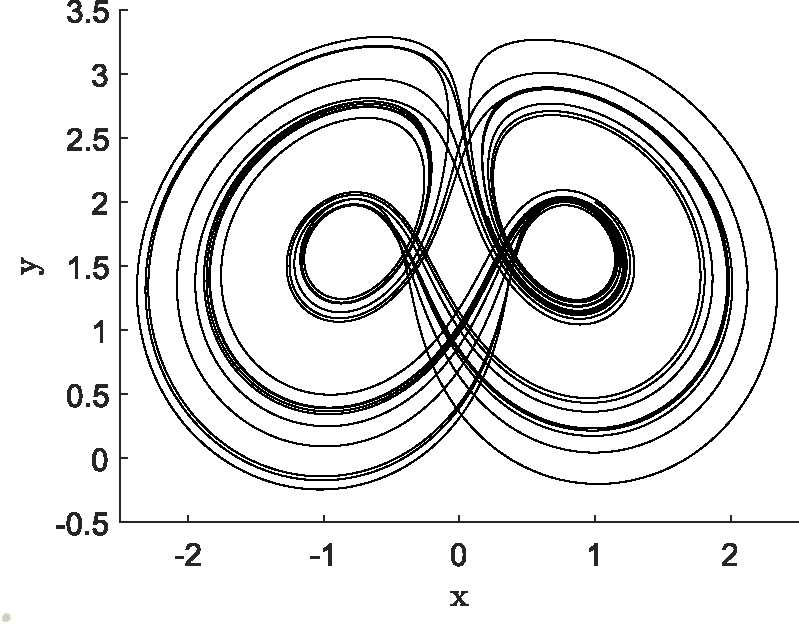
\includegraphics[scale=0.28]{files/int_adams_xy.pdf}
\end{subfigure}
\begin{subfigure}[ht]{0.3\textwidth}
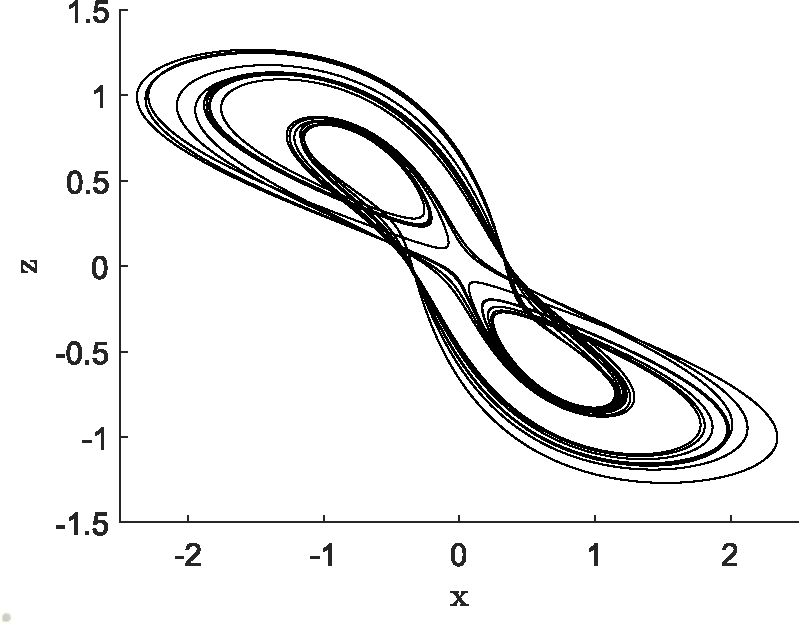
\includegraphics[scale=0.28]{files/int_adams_xz.pdf}
\end{subfigure}
\begin{subfigure}[ht]{0.3\textwidth}
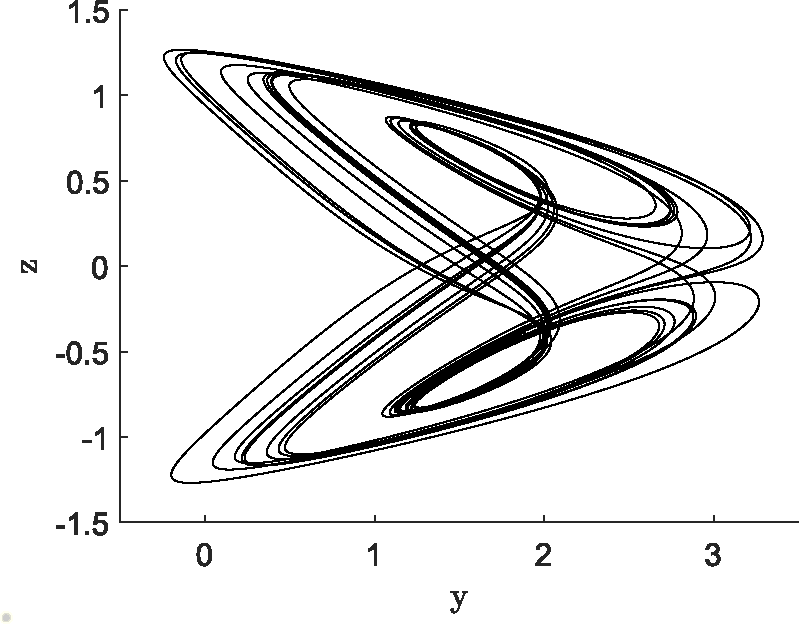
\includegraphics[scale=0.28]{files/int_adams_yz.pdf}
\end{subfigure}
\caption{Simulation Results: phase portraits.}
\label{fig:financeValidation}
\end{figure}
Now, in order to make a further validation of the presented algorithm, we will illustrate an example with a fractional initial value problem.
\begin{exmp}\label{ex:adam}
Solve the following the fractional initial value problem using ABM, with $y(0) = 1$ and $y'(0) = 0$.
\begin{equation}
    \mathcal{D}_c^{1.25}y(t)=-y(t)
\end{equation}
\end{exmp}
Carrying out some analytic operations, the exact solution is given by
\begin{equation}
    y(t) = E_{1.25,\,1}(-t^{1.25})=\sum_{k=0}^{\infty}\dfrac{(-1)^kt^{1.25k}}{\Gamma(1.25k +1)} 
\end{equation}
The ABM method was executed with different time-steps $h$ in order to show how the exact solution is better approximated for smaller values of $h$. The plot for the results are shown in figure \ref{fig:exAdams}; on the other hand, table \ref{tab:exAdams} shows the numeric approximation in certain values of $t$. Note that all approximations stabilize around the same value.
\begin{table}[H]
\centering
\begin{tabular}{cccccc}
\hline
\textbf{Time}    & \boldmath{$h=0.5$} & \boldmath{$h=0.25$} & \boldmath{$h=0.1$} & \boldmath{$h=0.01$} & \textbf{Exact}   \\ \hline
\boldmath{$t=0$} & 1                  & 1                   & 1                  & 1                   & 1       \\
\boldmath{$t=1$} & 0.0144             & 0.2147              & 0.3096             & 0.3601              & 0.3655  \\
\boldmath{$t=2$} & -0.1288            & -0.0527             & -0.0174            & 0.0016              & 0.0036  \\
\boldmath{$t=3$} & -0.1182            & -0.1065             & -0.1018            & -0.0992             & -0.0989 \\
\boldmath{$t=4$} & -0.0773            & -0.0854             & -0.0899     & -0.0923             & -0.0926 \\
\boldmath{$t=5$} & -0.0454            & -0.0547             & -0.0596            & -0.0622             & -0.0625 \\
\boldmath{$t=6$} & -0.0274            & -0.0335             & -0.0366            & -0.0383             & -0.0385 \\
\boldmath{$t=7$} & -0.0188            & -0.0221             & -0.0236            & -0.0245             & -0.0246 \\ \hline
\end{tabular}
\caption{Numerical results using ABM algorithm for different step sizes.}
\label{tab:exAdams}
\end{table}
\begin{figure}[H]
    \centering
    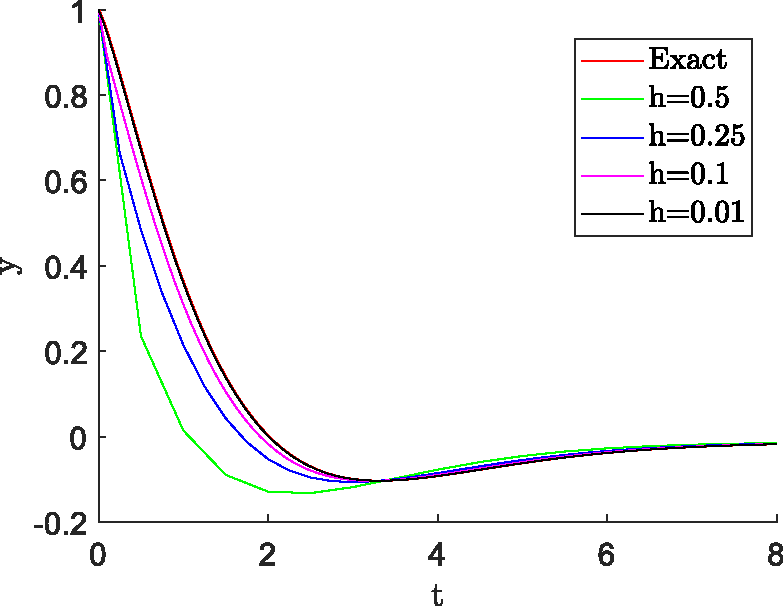
\includegraphics[scale=0.5]{files/ejemplo_adam.pdf}
    \caption{Results for different step-sizes using ABM predictor-corrector.}
    \label{fig:exAdams}
\end{figure}

\begin{exmp}
Chua Fractional System
\end{exmp}

The Chua system is given by:
\begin{equation}
    \begin{cases}
        \mathcal{D}_c^\alpha x(t) = a\left[x_2(t)-x_1(t)-f(x_1)\right]&\\
        \mathcal{D}_c^\alpha y(t) = x_1(t)-x_2(t)+x_3(t)&\\
        \mathcal{D}_c^\alpha z(t) = -bx_2(t)-cx_3(t)
    \end{cases}
\end{equation}
In our case, in order to compare with the results obtained in \cite{yang2018generation}, $\alpha=0.95$, $a=10.725$, $b=10.593$, $c = 0.268$, $m0 = -1.1726$, $m1 = -0.7872$ and
\begin{equation*}
    f(x_1)=m_1x_1(t)+\dfrac{1}{2}(m_0+m_1)\left(|x_1(t)+1|-|x_1(t)-1|\right)
\end{equation*}
with initial conditions $(x_0,\,y_0,\,z_0)=(-0.2,\, -0.1,\, 0.1)$, obtaining the following results:

\begin{figure}[H]
\centering
\begin{subfigure}[ht]{0.45\textwidth}
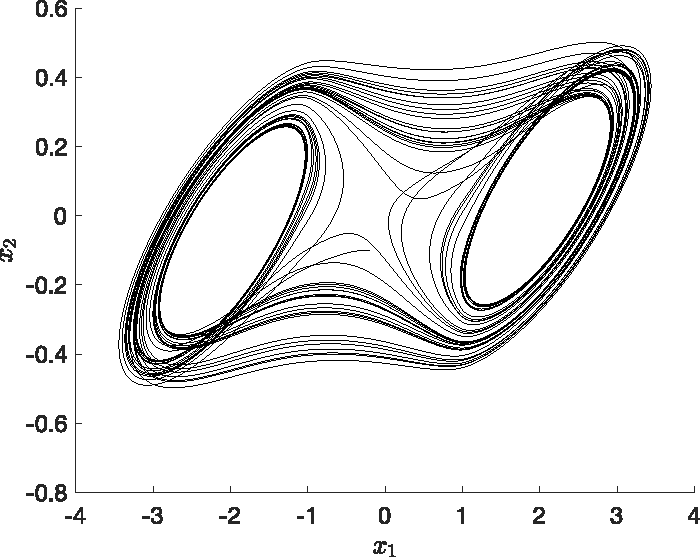
\includegraphics[scale=0.4]{files/ChuaX2vsX1_q0-95.pdf}
\end{subfigure}
\begin{subfigure}[ht]{0.45\textwidth}
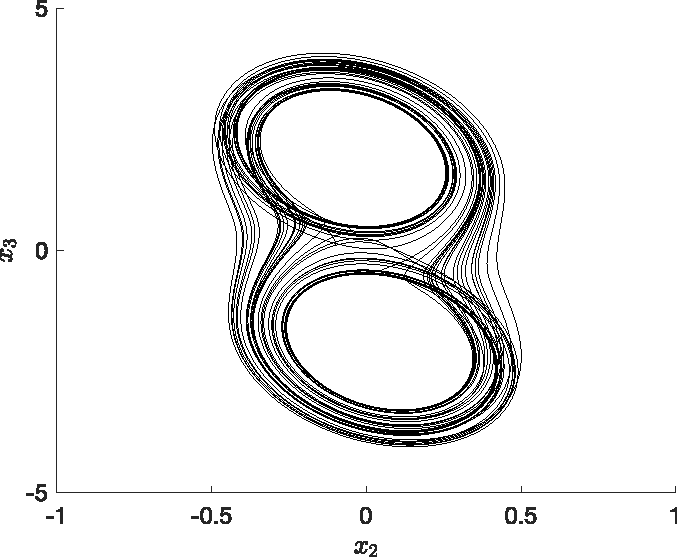
\includegraphics[scale=0.4]{files/ChuaX2vsX3_q0-95.pdf}
\end{subfigure}
\caption{Fractional Chua system: phase planes.}
\label{fig:Exchua}
\end{figure}

Which can be directly compared with figure 3 of Yang \textit{et al.} in \cite{yang2018generation}, obtaining the same results.

\begin{exmp}\label{ex:adam_disp}
ABM with explicit time
\end{exmp}

Solve the following initial value problem using ABM method, notice that in this problem the time is explicit in the differential equation.

\begin{equation} 
\mathcal{D}_{c}^{\alpha} y(t)= \frac{40320}{\Gamma(9-\alpha)} t^{8-\alpha}-3 \frac{\Gamma(5+\alpha / 2)}{\Gamma(5-\alpha / 2)} t^{4-\alpha / 2}+\frac{9}{4} \Gamma(\alpha+1)+\left(\frac{3}{2} t^{\alpha / 2}-t^{4}\right)^{3}-[y(t)]^{3 / 2} 
\end{equation}

Carrying out some analytic operations, with $\alpha=1.25 , y(0) = 1$ and $y'(0)=0$ the exact solution is given by:

\begin{equation}
    y(t) = t^{8}-3 t^{4+\alpha /2}+\frac{9}{4} t^{\alpha}
\end{equation}

The ABM, was performed with a step-size of $h=0.004$. In the figure \ref{fig:adam_disp}, it is shown a comparison between the exact solution and ABM, it can been that the numerical solution overlaps the exact solution, during the most of the simulation. It is important to remark that is a small time of simulation.

\begin{figure}[H]
    \centering
    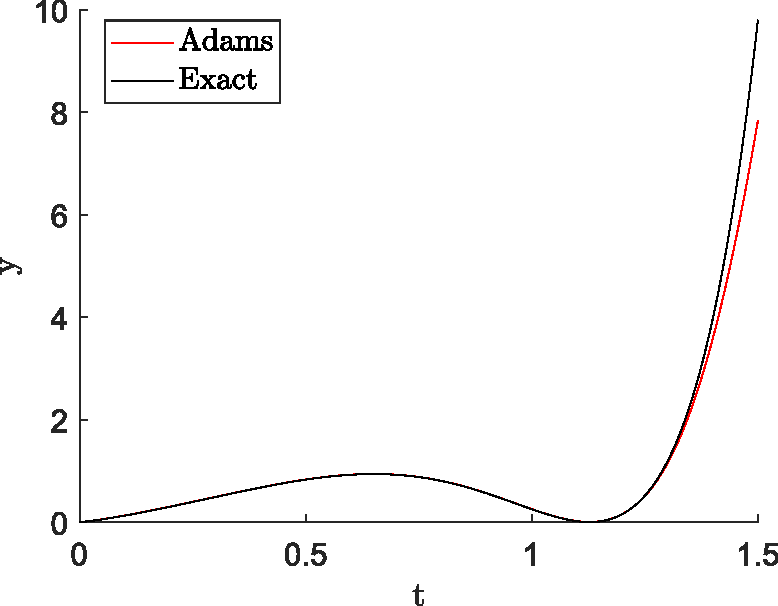
\includegraphics[scale=0.5]{files/adams_exact_xt_with_dispersion.pdf}
    \caption{ABM for fractional differential equations with explicit time, $T=1.5$.}
    \label{fig:adam_disp}
\end{figure}

In the figure \ref{fig:adam_disp2}, the time of the simulation was doubled, this clearly shows that when the time is explicit the behaviour of the numerical method diverges for big time of simulation, also is important to say that a comparison to the previous figure it is not valid to always assume that the performance of the system is going to continue approximating in a good way to the exact solution.

\begin{figure}[H]
    \centering
    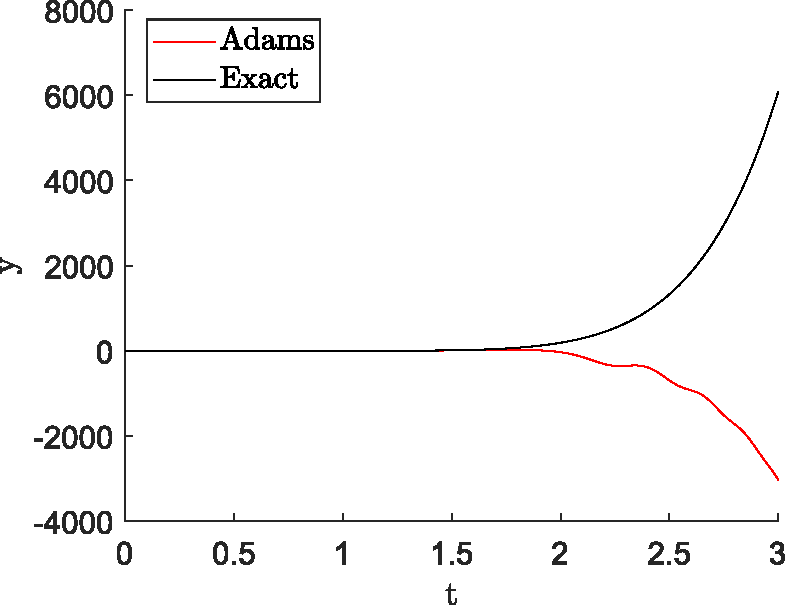
\includegraphics[scale=0.5]{files/adams_dispersion_2.pdf}
    \caption{ABM for fractional differential equations with explicit time, $T=3$.}
    \label{fig:adam_disp2}
\end{figure}


\subsection{Decomposition}
\subsubsection{Method}
Given a system of FDE
\begin{equation}
\begin{cases}
    \mathcal{D}_c^\alpha y(t)=f(t,y)&\\ y(0)=y_0\quad t\in[0,T]&
\end{cases}
\end{equation}\label{eq:FDESystemDeco}
the Adomian Decomposition method for fractional differential equations, presented in \cite{momani2007numerical}, starts by splitting $f$ as follows
\begin{equation}
    f(t,y)=g(t)+\mathbf{A}y+h(t,y)
\end{equation}
Where $g$ is the part of each equation that only depends on $t$; $\mathbf{A}y$ is the linear components of the equations and $h$ is the nonlinear part. Applying the Riemann-Liouville operator (section \ref{sec:RL}) to both sides of equation \ref{eq:FDESystemDeco}, we obtain
\begin{equation*}
    J^\alpha\mathcal{D}_c^\alpha y(t)=J^\alpha g(t)+J^\alpha\mathbf{A}y+J^\alpha h(t,y)
\end{equation*}
The left side of the equation can be calculated using theorem \ref{theo:rightinverse}. Therefore
\begin{equation*}
    y(t) = \sum_{r=0}^{m-1}\dfrac{y_{(r)}t^r}{r!}+ J^\alpha g(t)+J^\alpha\mathbf{A}y+J^\alpha h(t,y)
\end{equation*}
Since $\mathbf{y}$ is an unknown vector of solutions, it is approximated through a power series of functions as follows:
\begin{equation*}
    y(t)=\sum_{r=0}^\infty x_r(t)
\end{equation*}
That yields the next recursive scheme:
\begin{equation}\label{eq:recur_deco}
    \begin{split}
        x_0&=\sum_{r=0}^{m-1}\dfrac{y_{(r)}t^r}{r!}+J^\alpha g(t)\\
        x_{k+1}&=J^\alpha \mathbf{A}x_k+J^\alpha \tilde{h}_k\left(t,\sum_{r=0}^kx_j(t)\right)
    \end{split}
\end{equation}
Where $\tilde{h}_k$ is the Adomian polynomial, described by
\begin{equation}
    \tilde{h}_k\left(t,\sum_{r=0}^{k}x_j(t)\right)=\dfrac{1}{k!}\left[\dfrac{d^k}{d\lambda^k}h\left(t,\sum_{j=0}^{k}\lambda^jx_j(t)\right)\Bigg|_{\lambda=0}\right]
\end{equation}


\begin{exmp}\label{ex:deco}
Solve the following the fractional initial value problem using Decomposition, with $y(0)=1$ and $y'(0)=0$.
\begin{equation}
    \mathcal{D}_c^{1.25}y(t)=-y(t)
\end{equation}
\end{exmp}
Carrying out some analytic operations, the exact solution is given by
\begin{equation}
    y(t) = E_{1.25,\,1}(-t^{1.25})=\sum_{k=0}^{\infty}\dfrac{(-1)^kt^{1.25k}}{\Gamma(1.25k +1)} 
\end{equation}
Notice that this example is the same as the one that was developed in the previous section: example \ref{ex:adam}.

The Decomposition method was executed with different number of polynomials in order to show how the exact solution is better approximated for more polynomials. The plot for the results are shown in figure \ref{fig:deco_frac}; on the other hand, table \ref{tab:exDeco} shows the numeric approximation in certain values of $t$. Note that all approximations stabilize around the same value.

\begin{table}[H]
\centering
\begin{tabular}{cccccc}
\hline
\textbf{Time}    & \boldmath{$N=1$} & \boldmath{$N=5$} & \boldmath{$N=10$} & \boldmath{$N=15$} & Exact   \\ \hline
\boldmath{$t=0$} & 1.0000           & 1.0000           & 1.0000            & 1.0000            & 1.0000  \\
\boldmath{$t=1$} & 0.1174           & 0.3655           & 0.3655            & 0.3655            & 0.3655  \\
\boldmath{$t=2$} & -1.0992          & -0.0074          & 0.0036            & 0.0036            & 0.0036  \\
\boldmath{$t=3$} & -2.4847          & -0.3103          & -0.0988           & -0.0989           & -0.0989 \\
\boldmath{$t=4$} & -3.9928          & -1.7581          & -0.0891           & -0.0926           & -0.0926 \\
\boldmath{$t=5$} & -5.5990          & -8.1585          & 0.0098            & -0.0625           & -0.0625 \\
\boldmath{$t=6$} & -7.2882          & -29.0799         & 0.8027            & -0.0397           & -0.0385 \\
\boldmath{$t=7$} & -9.0494          & -84.6072         & 6.6218            & -0.0508           & -0.0246 \\ \hline
\end{tabular}
\caption{Numerical results using Decomposition algorithm for different polynomials}
\label{tab:exDeco}
\end{table}

\begin{figure}[H]
    \centering
    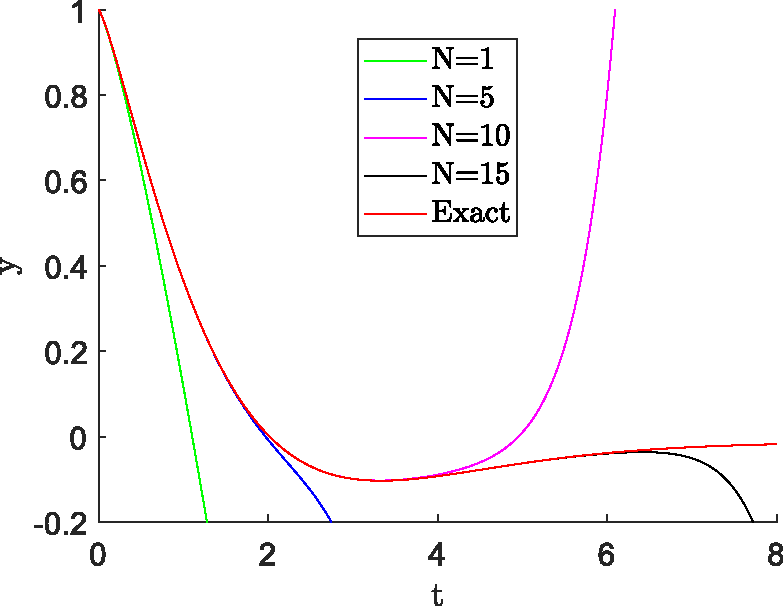
\includegraphics[scale=0.5]{files/frac_deco.pdf}
    \caption{Decomposition using different number of polynomials.}
    \label{fig:deco_frac}
\end{figure}

\subsection{Phase Variables: Fractional Case}
Suppose we have the multi-term fractional differential equation
\begin{equation}
    \begin{cases}
    \mathcal{D}_c^{\alpha_n}y(t)=f\left(t,y,\mathcal{D}_c^{\alpha_1}y,\mathcal{D}_c^{\alpha_2}y,\dots,\mathcal{D}_c^{\alpha_{n-1}}y\right)&\\
    y(0)=y_0,\,\dots,y^{(m-1)}(0)= y_{(m-1)}\quad t\in[0,T]
    \end{cases}
\end{equation}
    where $m=\ceil{\alpha_n}$ and $0<\alpha_{1}<\alpha_{2}<\ldots<\alpha_{n}$. We select new orders $\tilde{\alpha}_{1}, \ldots, \tilde{\alpha}_{n}$ such that
    \[\begin{array}{l}{\text { (a) } \tilde{\alpha}_{1}, \ldots, \tilde{\alpha}_{n} \text { must be rational numbers, }} \\ {\text { (b) }\left\lceil\alpha_{n}\right\rceil=\left\lceil\tilde{\alpha}_{n}\right\rceil} \\ {\text { (c) } \operatorname{gcd}\left(1, \tilde{\alpha}_{1}, \ldots, \tilde{\alpha}_{n}\right) \text { should be as large as possible, }} \\ {\text { (d) }\left|\alpha_{j}-\tilde{\alpha}_{j}\right| \text { should be as small as possible for all } j}\end{array}\]

    We build the approximated system of FDEs with \[\gamma :=\operatorname{gcd}\left(1, \tilde{\alpha}_{1}, \ldots, \tilde{\alpha}_{n}\right)\qquad\tilde{N} :=\frac{\tilde{\alpha}_{n}}{\gamma}\]
    \begin{equation}
    \begin{cases}
    
    \mathcal{D}_c^{\gamma} x_{0} =x_{1} &\\[5pt]
    \mathcal{D}_c^{\gamma} x_{1} =x_{2} &\\
    \qquad\vdots &\\
    \mathcal{D}_c^{\gamma} =x_{\tilde{N}-1} &\\[5pt]
    \mathcal{D}_c^{\gamma} =f\left(t, x_{0}, x_{\tilde{\alpha}_{1} / \gamma}, \ldots, x_{\tilde{\alpha}_{n-1} / \gamma}\right) \end{cases}
    \end{equation}
    \begin{equation}
    x _ { j } ( 0 ) = \begin{cases} { y _ { ( j \gamma ) }   } & { \text { for } j \gamma \in \mathbb { N } _ { 0 } } \\ { 0  } & { \text { else } } \end{cases}
    \end{equation}



\section{Method Comparison}
In the following sections, the methods explained previously are going to be compared for multiple examples. First, the integer-order algorithms and ABM for some integer-order systems and then a comparison of the fractional algorithms is performed. 

\subsection{Integer models}
Ensuing, four examples for integer systems of ODEs are presented, in order to compare ABM, Euler and RK4.
\subsubsection{Chaotic Financial System}
Recall the example \ref{ex:finance}. This system will now be compared with the Adams-Bashforth-Moulton predictor-corrector algorithm for an integer system of ODEs. The results of this simulation are presented in figure \ref{fig:comparFinanceX}.

\begin{figure}[H]
    \centering
    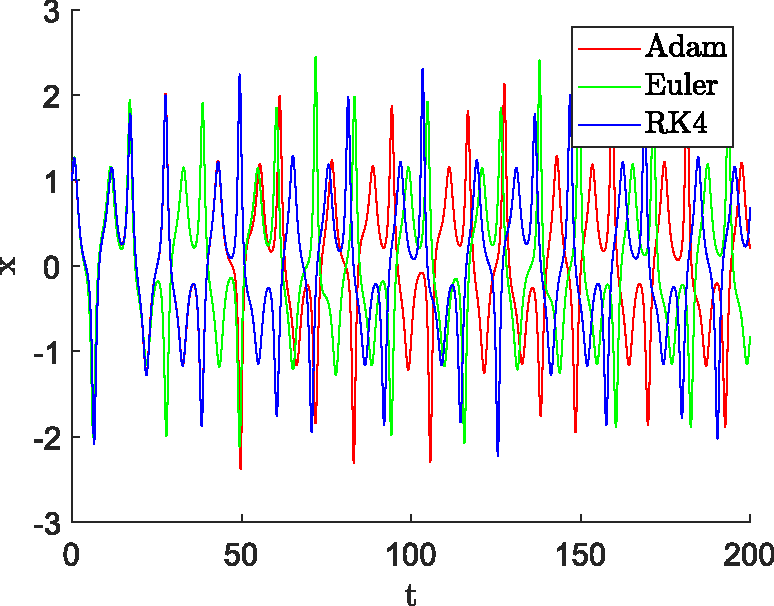
\includegraphics[scale=0.5]{files/adm_euler_rk4_x.pdf}
    \caption{}
    \label{fig:comparFinanceX}
\end{figure}



\subsubsection{Thomas' Cyclically Symmetric Attractor}
This system was originally proposed by R. Thomas in \cite{thomas1999deterministic}. It describes a deterministic fractional Brownian motion, this system can be used to model auto-catalytic chemical reactions, ecology and evolution systems. The parameter $b$ represents the frictional damping for a particle moving in a 3D labyrinth \cite{sprott2007labyrinth}. This dynamic system is given by
\begin{equation}
    \begin{cases}
        x'=\sin(y)-bx&\\
        y'=\sin(z)-by&\\
        z'=\sin(x)-bz&\\
    \end{cases}
\end{equation}

The following simulations were performed with initial conditions $(x_0,\,y_0,\,z_0)=(0,\,0.1,\,0)$ and $b=0.18$; each figure shows the state variables through time, where it was use three different numeric methods to solve the system. For the ABM predictor-corrector, $\alpha=1$ since it is a system of integer ordinary differential equations
\begin{figure}[H]
\centering
\begin{subfigure}[ht]{0.3\textwidth}
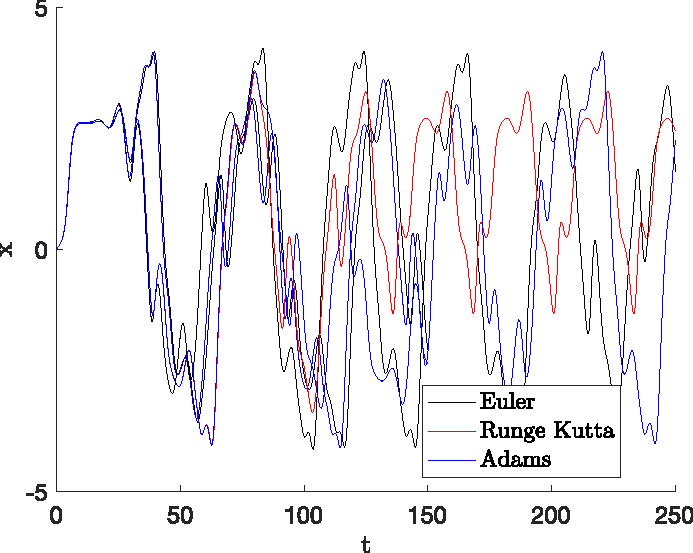
\includegraphics[scale=0.33]{files/ThomasXvsT.pdf}
\end{subfigure}
\begin{subfigure}[ht]{0.3\textwidth}
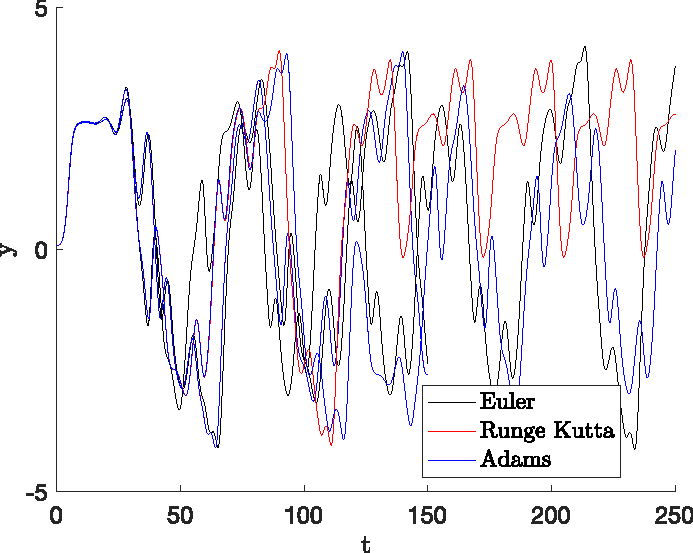
\includegraphics[scale=0.33]{files/ThomasYvsT.pdf}
\end{subfigure}
\begin{subfigure}[ht]{0.3\textwidth}
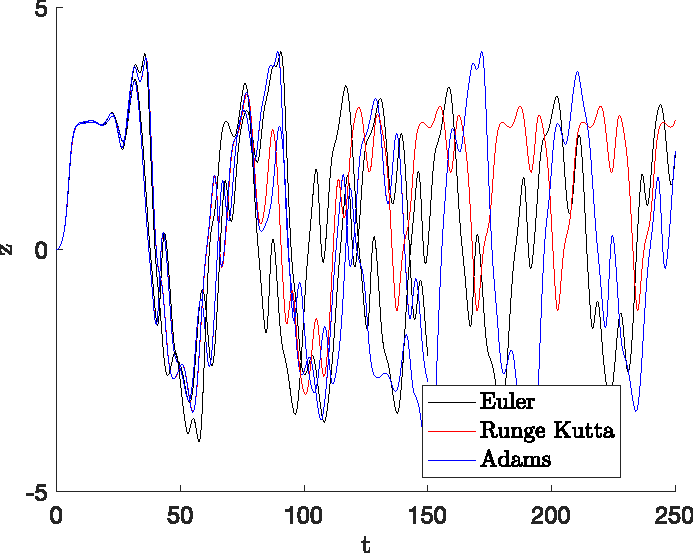
\includegraphics[scale=0.33]{files/ThomasZvsT.pdf}
\end{subfigure}
\caption{}
\label{fig:thomasExample}
\end{figure}

The 3D portrait of the Thomas' system is shown in figure \ref{fig:thomas3d}.
\begin{figure}[H]
    \centering
    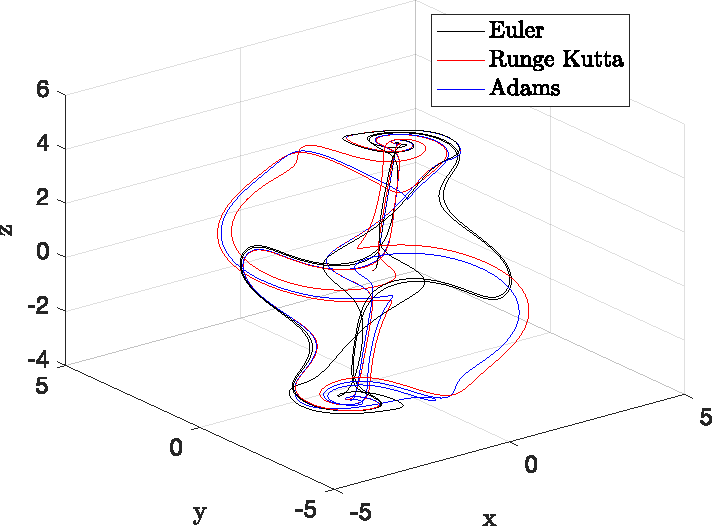
\includegraphics[scale=0.6]{files/3DThomas.pdf}
    \caption{3D phase portrait for the Thomas' system.}
    \label{fig:thomas3d}
\end{figure}

In order to compare Euler, RK4 and ABM methods, we present the results in figure \ref{fig:thomasExample}. It can be easily seen that in the beginning of the simulation the three solutions has similar behavior. Lately, the three solutions diverge compared to each other, but RK4 and ABM, stay more time with similar behavior. The discrepancies are possible due to the different calculations that each method needs, carrying his own errors. Other important fact to have into account, is that we are simulating a chaotic system, so small changes generate big differences in the future.


\subsubsection{Langford (Aizawa) Attractor}
The following set of differential equations were proposed by W. F. Langford in \cite{langford1984numerical}. This system is often called the Aizawa Attractor. 
\begin{equation}
    \begin{cases}
        x'=(z-\beta)x-\omega y&\\
        y'=\omega x+(z-\beta)y&\\
        z'=\lambda+\alpha z-\dfrac{z^3}{3}-(x^2+y^2)(1+\rho z)+\epsilon zx^3&\\
    \end{cases}
\end{equation}
The following simulations were performed with initial conditions $(x_0,\,y_0,\,z_0)=(0.1,\,0,\,0)$ and $\alpha=0.95$, $\beta=0.7$, $\lambda=0.6$, $\omega=3.5$, $\rho=0.25$ and $\epsilon=0.1$; each figure shows the state variables through time, where it was use three different numeric methods to solve the system. For the ABM predictor-corrector, $\alpha=1$ since it is a system of integer ordinary differential equations.
\begin{figure}[H]
\centering
\begin{subfigure}[b]{0.4\textwidth}
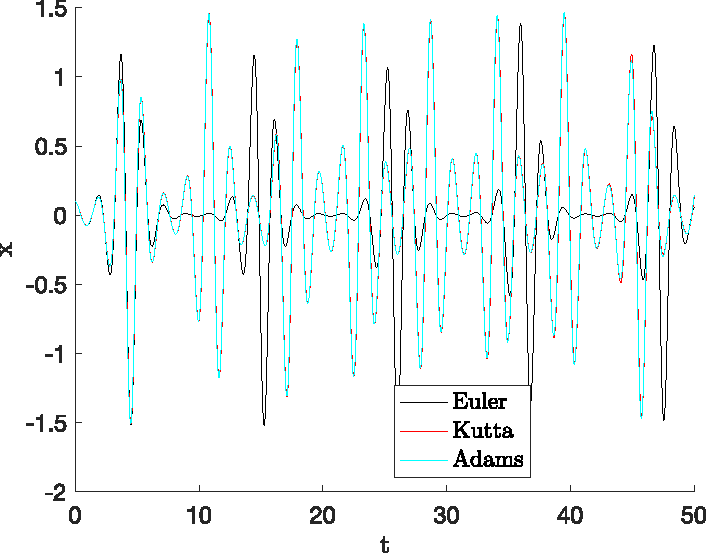
\includegraphics[scale=0.45]{files/AizawaXvsT.pdf}
\end{subfigure}
\hspace{1.5cm}
\begin{subfigure}[b]{0.4\textwidth}
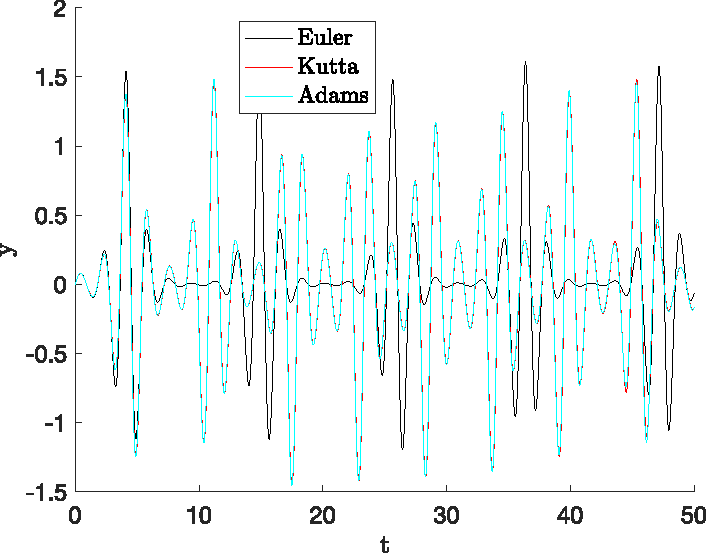
\includegraphics[scale=0.45]{files/AizawaYvsT.pdf}
\end{subfigure}
\vskip\baselineskip
\begin{subfigure}[b]{0.4\textwidth}
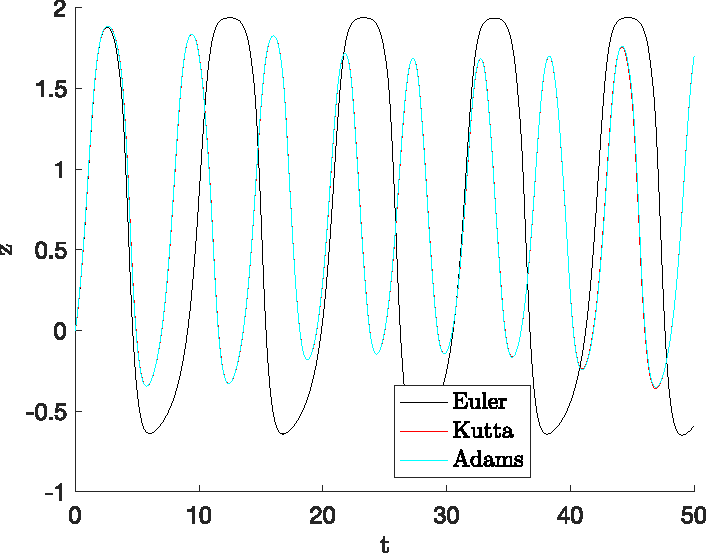
\includegraphics[scale=0.45]{files/AizawaZvsT.pdf}
\end{subfigure}
\caption{State variables response in time.}
\label{fig:aizawaExample}
\end{figure}

\begin{figure}[H]
    \centering
    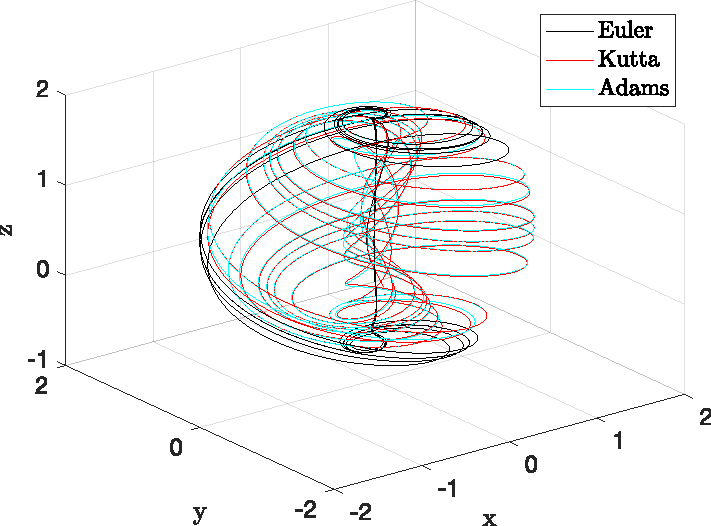
\includegraphics[scale=0.5]{files/3DIntegerAizawa.pdf}
    \caption{3D phase portrait for the Aizawa's system.}
    \label{fig:aizawa3d}
\end{figure}

With the Aizawa's systems occurs something similar with what we have already discussed in the previous section, with the difference that ABM and RK4 stayed together, overlapping the signals during the simulation except in the time series of the state variable $y$ approximately in the time 45, where RK4 has a lower peak proving that, effectively, RK4 and ABM overlap.

\subsubsection{Integer order systems}\label{subsec:int_ord}

Solve the following set of differential equations, using Euler, RK4, ABM and Decomposition, with the initial conditions $x(0) = 1, y(0) = -1$.

\begin{equation}
    \begin{cases}
        x'= y&\\
        y'= 2x - y&\\
    \end{cases}
\end{equation}

Carrying out some analytic operations, the exact solution is given by:

\begin{equation}
    \begin{cases}
        x = \dfrac{1}{3}e^{-2t}(e^{3t}+2)&\vspace{2mm}\\
        y = 
        \dfrac{1}{3}e^{-2t}(e^{3t}-4)&\\
    \end{cases}
\end{equation}

In the figure \ref{fig:int_todos} is compare the exact solution with decomposition, RK4, Euler and ABM.

\begin{figure}[H]
    \centering
    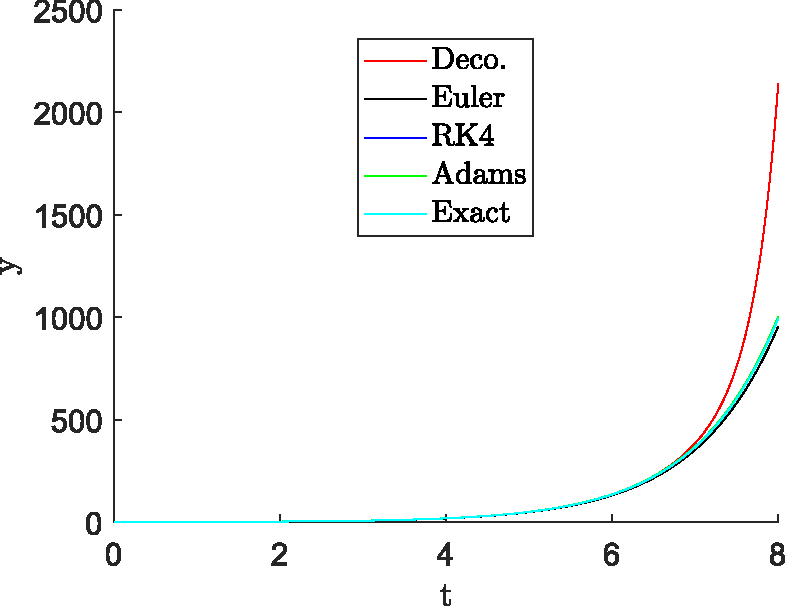
\includegraphics[scale=0.5]{files/int_todos.pdf}
    \caption{Results using different methods.}
    \label{fig:int_todos}
\end{figure}

It can be easily seen that during the simulation all the methods overlap the exact solution, except Decomposition (red signal) that in the time seven, it starts increase more than the other ones, because even though this method gives an analytical solution, it use a polynomial with infinite terms, so it´s necessary to truncate it in some point and then is when it diverges compare with the exact solution.

\subsection{Fractional models}
Subsequent, it is presented some examples SOMEEEEEEEEEEEEEEEEEEEEEEEEEEEEEEEEEEEEEEEEEE OR ONE??????????????????????????????????????????????????????????????????? to compare the fractional methods with the exact solution, i.e Decomposition and ABM.

\subsubsection{ABM and decomposition}

In order to compare Decomposition and ABM, it was solved the following the fractional initial value problem, with $y(0) = 1$ and $y'(0)=0$. Notice that is the same example present on each method (for ABM example \ref{ex:adam} and for Decomposition \ref{ex:deco}). 
\begin{equation}
    \mathcal{D}_c^{1.25}y(t)=-y(t)
\end{equation}
Carrying out some analytic operations, the exact solution is given by
\begin{equation}
    y(t) = E_{1.25,\,1}(-t^{1.25})=\sum_{k=0}^{\infty}\dfrac{(-1)^kt^{1.25k}}{\Gamma(1.25k +1)}
\end{equation}

In order to obtain a numerical solution Decomposition was performed with $15$ polynomial terms and ABM with a step-size $h=0.01$. Analyzing the figure \ref{fig:abm_decomp}, it can easily seen that it happen the same as in the comparison of the methods, in the previous section, i.e \ref{subsec:int_ord}. 

Both numerical solutions overlap the most of the simulation, but in a specific time, approximately at 7 is when Decomposition did not stabilize as the other ones, this is due to the truncation use in the method.


\begin{figure}[H]
    \centering
    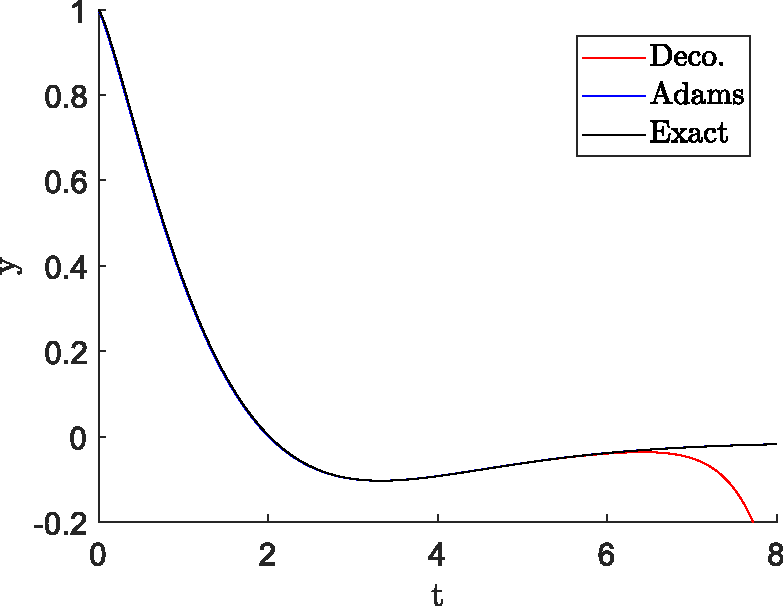
\includegraphics[scale=0.5]{files/adams_exact_deco.pdf}
    \caption{Results using ABM and decomposition}
    \label{fig:abm_decomp}
\end{figure}


OTROOOOOOOOOOOOOOOOOOOOOOOOOOOOOOOOOOOOOOOOOOOOOOOOOOOOOOOOOOOOOOOOOOOOOOOOOOOOOO EJEMPLOOOOOOOOOOOOOOOOOOOOOOOOOOOOOOOOOOOOOOOOOOOOOOOO




\chapter{Algorithm Modifications}\label{chap:modif}
\section{Predicted-Variation of ABM} \label{sec:predABM}
As seen in section \ref{sec:ABM}, the ABM method needs to use a predicted value for every iteration; therefore, only if the solution converges, the value of $y$ that you obtained could be used as another predicted value for the variable and use it to obtain a more precise solution. So, the algorithm could keep doing this till the difference of the last predicted values reaches a small $\epsilon$ picked by the user or as it reaches a maximum iteration, so it is certain that the algorithm always terminates.

This modification does increase the accuracy (to which extent, it is gonna be discussed in this section) but it increases the run time of the method. 

\subsection{Chaotic Financial System}
In order to test this modification, the Financial System studied in example \ref{ex:finance} will be tested. The respective generalization to fractional-order differential equations, following \cite{chen2008nonlinear}, will be
\begin{equation}
    \begin{cases}
    \mathcal{D}_c^{\alpha_1} x=z+(y-a)x&\\
    \mathcal{D}_c^{\alpha_2} y=1-by-x^2&\\
    \mathcal{D}_c^{\alpha_3} z=-x-cz&
    \end{cases}
\end{equation}

The simulations were performed using $(\alpha_1,\,\alpha_2,\,\alpha_3)=(1,\,1,\, 0.8)$, $(x_0,\,y_0,\,z_0)=(2,\,3,\,2)$, $T=200$ and $N=10000$. The parameters were chosen as $(a,\,b,\,c)=(3,\,0.1,\,1)$, in order to compare the results with \cite{chen2008nonlinear}. The simulations are shown in the following figures (\ref{fig:predictedFinancial} for time-series and \ref{fig:predictedFinancialXY} for $XY$ phase portrait):

\begin{figure}[H]
\centering
\begin{subfigure}[ht]{0.3\textwidth}
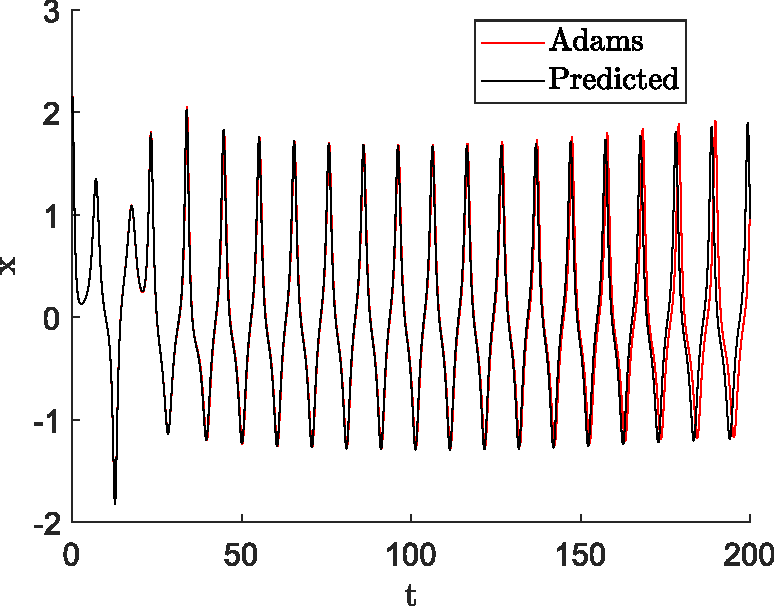
\includegraphics[scale=0.29]{files/adams_predicted_tx.pdf}
\end{subfigure}
\begin{subfigure}[ht]{0.3\textwidth}
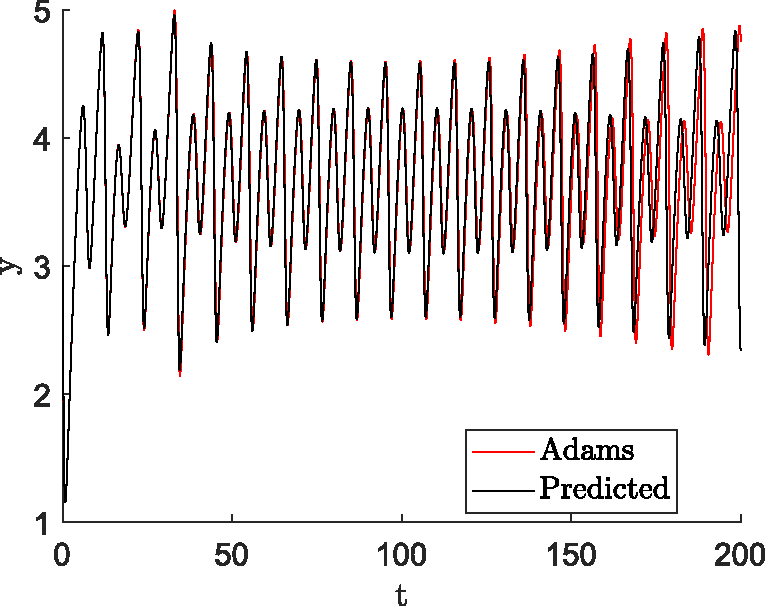
\includegraphics[scale=0.29]{files/adams_predicted_ty.pdf}
\end{subfigure}
\begin{subfigure}[ht]{0.3\textwidth}
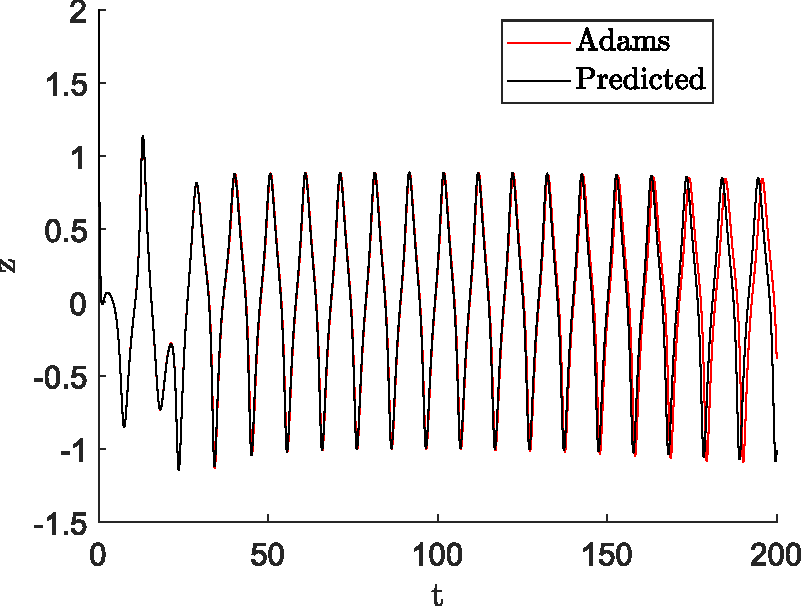
\includegraphics[scale=0.29]{files/adams_predicted_tz.pdf}
\end{subfigure}
\caption{Predicted modification compared with the original algorithm.}
\label{fig:predictedFinancial}
\end{figure}

\begin{figure}[H]
    \centering
    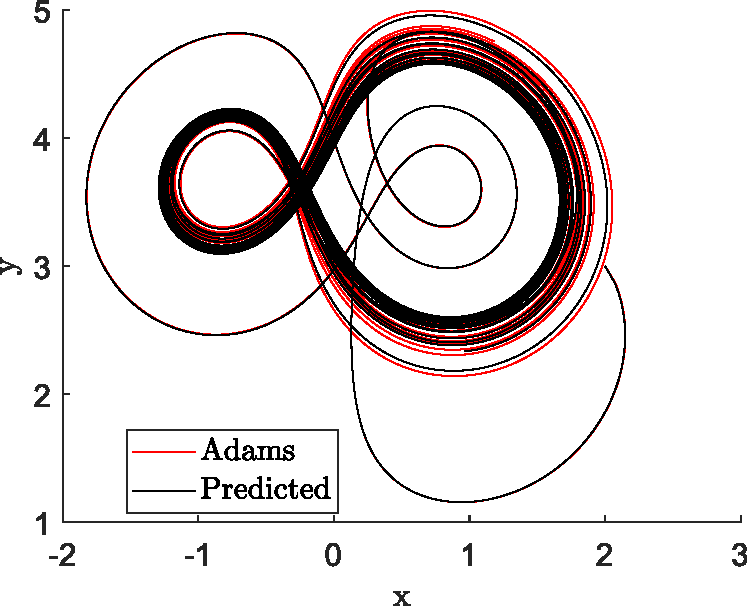
\includegraphics[scale=0.5]{files/adams_predicted_xy.pdf}
    \caption{Phase plane for the variables x and y.}
    \label{fig:predictedFinancialXY}
\end{figure}
This results show that this modification does not show significant improvement in this particular example. In figure \ref{fig:predictedFinancial}, the time series are shown for all state variables $x$, $y$ and $z$; note that both approximations overlap (generally). 

\subsection{Bagley-Torvik Equation}
The Bagley-Torvik equation is a model the describes the motion of a rigid plate in a Newtonian fluid, this equation was originally proposed in \cite{torvik1984appearance}. This model is given by
\begin{equation}
    Ay''(t)+B\mathcal{D}_c^{3/2}y(t)+Cy(t)=f(t)
\end{equation}

As Diethelm and Ford states in \cite{diethelm2002numerical}, if $f(t)=1+t$, the exact solution to this problem is given by
\begin{equation}
    y(t)=1+t
\end{equation}
For any choice of parameters $A$, $B$ and $C$.

Now we will use this result as a reference to compare the ABM method and the modification presented in this section. Following the ideas presented in section PHASE FRACTIONAL

The simulation was conducted based on \cite{diethelm2002numerical}, therefore, we chose $A=B=C=1$. The simulation was conducted, for the standard ABM method, with $T=10$, $N=15$; and, for the predicted scheme, with $T=10$, $N=15$, $\text{\texttt{tol}}=10^{-7}$ and $\text{\texttt{nmax}}=10$. The results are presented in figure \ref{fig:comparBagleyTorvik}.


\begin{figure}[H]
    \centering
    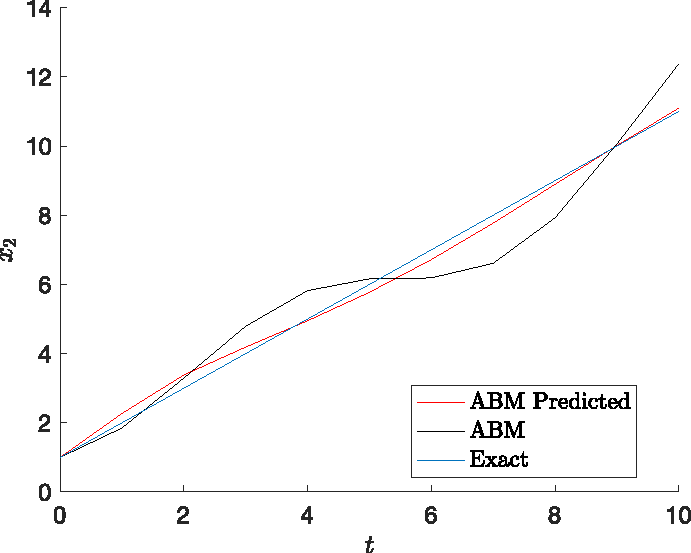
\includegraphics[scale=0.5]{files/comparPredictedABM.pdf}
    \caption{Comparison between the original and predicted scheme.}
    \label{fig:comparBagleyTorvik}
\end{figure}

\section{Quadrature Decomposition}
This suggestion is proposed to the decomposition method. Recall the recursive scheme (\ref{eq:recur_deco}) that was obtained in for approximating the solution; the idea of this experiment is based on the fact that the solution is approximated in terms of the Riemann-Liouville integral for an unspecified time $t$. This implies that the approximation is a function of $t$ and it could be approximated for each point on the partitioned interval $[0,T]$; this means that the Riemann-Liouville integral would no longer be a function of $t$ and it would rather be an standard definite integral, which can be approximated using classical quadrature rules (trapezoidal or Simpson rules).

In order to test the proposed scheme, we will use the following integer system or ODEs, and the results are shown in figure \ref{fig:qDeco_ex}.
\begin{equation}
  \begin{cases}
    x'=y&x(0)=1\\
    y'=2x-y&y(0)=-1
  \end{cases}
\end{equation}

Clearly, this approach did not give a correct approximation, not even for an integer-order system of ODEs. This is due to the fact that the classical quadrature formulas do not take information about the complete history of the function but only taking some points (not even taking information about the polynomial in the previous step), losing important information about the past of the function and it is unable to make an accurate approximation. 

¿TIENE SENTIDO? Es un ode... no importa la memoria, ¿o sí?

\begin{figure}[H]
  \centering
  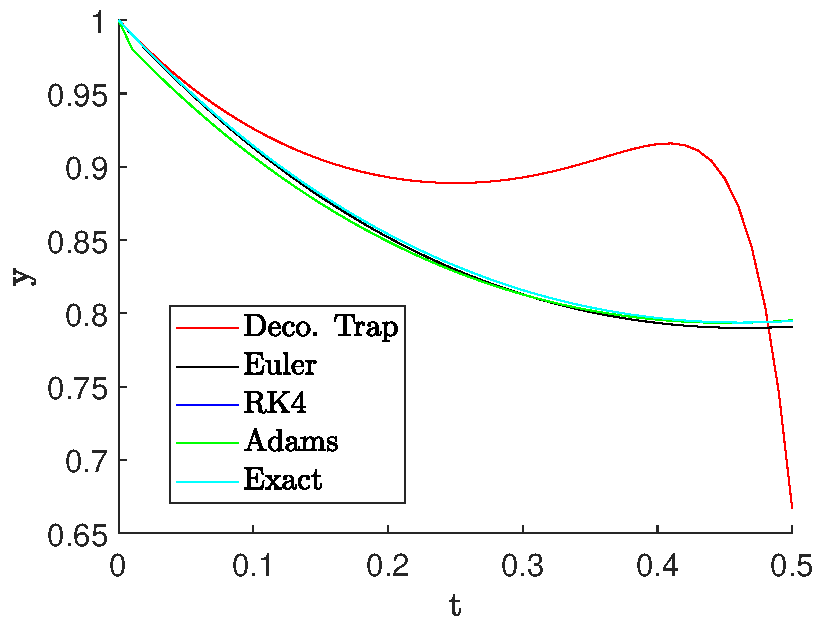
\includegraphics[scale=.5]{files/decom_trap.pdf}
  \caption{Results for quadrature decomposition.}
  \label{fig:qDeco_ex}
\end{figure}

\section{Polynomial Decomposition}
This approach is based on the simple computation of the Riemann-Liouville integral for real polynomials:
\begin{equation}
  J^{\alpha}\left(t^{\beta}\right)=\dfrac{\Gamma(\beta+1)}{\Gamma(\alpha+\beta+1)}t^{\alpha+\beta},\quad \alpha>0,\,\beta\in\mathbb{R}
\end{equation}
The main idea is to convert the right-hand side of the approximation with decomposition into polynomials, using polynomial interpolation techniques. This method is useful for non-chaotic fractional dynamic systems or chaotic ones for small time frames.

In order to validate the method, we present three different examples applying the depicted method.

Consider the following multi-term nonlinear fractional differential equation
\begin{equation}\label{ivp:pDeco}
    \begin{cases}
        y'''(t)+\mathcal{D}_c^{5/2}y(t)+y^2(t)=t^4&\\
        y(0)=y'(0)=0,\,y''(0)=2
    \end{cases}
\end{equation}
The exact solution to this FDE is $y(t)=t^2$ \cite{saadatmandi2010new}. The polynomial decomposition was applied and compared with the ABM method (figure \ref{fig:pDeco_exact}).

\begin{figure}
    \centering
    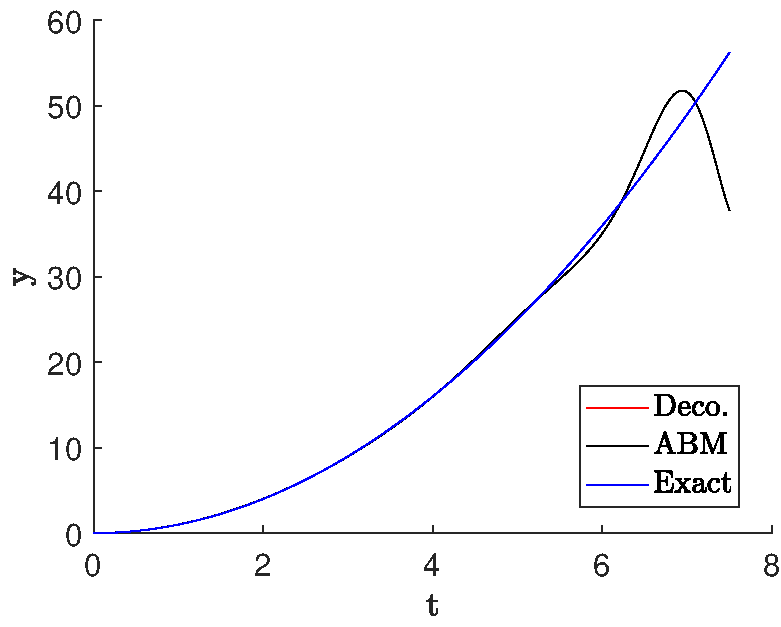
\includegraphics[scale=.5]{files/ABM-vs-Deco-Exact.pdf}
    \caption{Approximate solution to problem \ref{ivp:pDeco} using ABM and polynomial decomposition.}
    \label{fig:pDeco_exact}
\end{figure}

%\appendix



%https://www.mathworks.com/matlabcentral/fileexchange/24515-m-code-to-latex-converter

\nocite{*}
\bibliography{ref}
\bibliographystyle{IEEEtran}


\end{document}
